\documentclass{article}

\usepackage[nonatbib,final]{neurips}
\usepackage{afterpage}
\usepackage[backend=biber,style=numeric-comp,doi=false,url=false]{biblatex}
\setlength\bibitemsep{0.5\baselineskip}
\usepackage{bm}
\usepackage{csquotes}
\usepackage[inkscapelatex=false]{svg}

\newcommand{\CE}[2]{\text{CE}(#1 \mathrel{\Vert} #2)}

\addbibresource{references.bib}
\graphicspath{{../figs/}}
\svgpath{{../plots/}}

\newcommand{\todo}{\bf \color{blue} [TODO]~}

\makeatletter
\renewcommand{\@noticestring}{
  \centering

}
\makeatother

\usepackage[ruled]{algorithm2e}
\usepackage{hyperref}
\usepackage{microtype}
\usepackage{pifont}
\usepackage{xcolor}
\usepackage{xurl}
% Figures and Tables
\usepackage{graphicx}
\usepackage{booktabs, multirow}
% Monospaced Code Blocks
\usepackage{listings}
% Math Packages
\usepackage{amsmath, amsfonts, amsthm}
\usepackage{nicefrac}

\lstset{
  backgroundcolor=\color{white},   % choose the background color; you must add \usepackage{color} or \usepackage{xcolor}; should come as last argument
  basicstyle=\ttfamily,            % the size of the fonts that are used for the code
  breakatwhitespace=false,         % sets if automatic breaks should only happen at whitespace
  breaklines=true,                 % sets automatic line breaking
  captionpos=b,                    % sets the caption-position to bottom
  columns=fullflexible,            % reduce the column spacing
  commentstyle=\color{gray},       % comment style
  deletekeywords={},               % if you want to delete keywords from the given language
  escapeinside={\%*}{*)},          % if you want to add LaTeX within your code
  extendedchars=true,              % lets you use non-ASCII characters; for 8-bits encodings only, does not work with UTF-8
  frame=none,                      % adds no frame around the code
  keepspaces=true,                 % keeps spaces in text, useful for keeping indentation of code (possibly needs columns=flexible)
  keywordstyle=\color{blue},       % keyword style
  language=C++,                    % the language of the code
  morekeywords={},                 % if you want to add more keywords to the set
  numbers=none,                    % where to put the line-numbers; possible values are (none, left, right)
  numbersep=5pt,                   % how far the line-numbers are from the code
  numberstyle=\color{black},       % the style that is used for the line-numbers
  rulecolor=\color{black},         % if not set, the frame-color may be changed on line-breaks within not-black text (e.g. comments (green here))
  showspaces=false,                % show spaces everywhere adding particular underscores; it overrides 'showstringspaces'
  showstringspaces=false,          % underline spaces within strings only
  showtabs=false,                  % show tabs within strings adding particular underscores
  stepnumber=1,                    % the step between two line-numbers. If it's 1, each line will be numbered
  stringstyle=\color{red},         % string literal style
  tabsize=4,                       % sets default tabsize to 4 spaces
}

\newtheorem{theorem}{Theorem}[section]
\newtheorem{claim}[theorem]{Claim}
\newtheorem{lemma}[theorem]{Lemma}
\newtheorem{corollary}[theorem]{Corollary}
\newtheorem*{remark}{Remark}
\newtheorem*{example}{Example}


\usepackage{physics}
\usepackage{mathtools}
\DeclarePairedDelimiter\p{(}{)}
\DeclarePairedDelimiter\n{|}{|}
\DeclarePairedDelimiter\B{[}{]}

\title{Self-Training with Models for Tabular Data}

\author{
    Wei En, Ng \\
    National University of Singapore \\
    \texttt{\href{mailto:ngwe@u.nus.edu}{ngwe@u.nus.edu}}
}

\begin{document}

\maketitle

\tableofcontents

\section{Introduction}

This report details some preliminary experiments studying self-training
\cite{amini2023selftraining} on tabular data, where tree-based models often outperform
deep learning methods significantly in the typical supervised learning (SL) setting
\cite{shwartz-ziv2021tabular,grinsztajn2022why}.\footnote{%
  Some recent works \cite{gorishniy2023tabr} have claimed to develop deep learning
  models that can outperform tree-based methods such as XGBoost \cite{chen2016xgboost}
  on tabular data.
}

\paragraph{Background.}
Several observations have been made on the performance of these methods:
\begin{enumerate}
    \item ($\bm{-}$) Increasing the random search budget for hyperparameters does
    not benefit NNs. \cite{grinsztajn2022why}
    \item ($\bm{-}$) NNs continue to do poorly on datasets with only numerical
    features, although the performance gap is slightly reduced compared to datasets with
    categorical features. \cite{grinsztajn2022why}
    \item ($\bm{+}$) Increasing the number of training samples might reduce the
    performance gap. \cite{grinsztajn2022why}
\end{enumerate}

Furthermore, low-data regimes for tabular data do not appear to be well-studied,
possibly because tree-based models often reach near-optimal performance with low
training dataset sizes.\footnote{%
  See Figure \ref{fig:ul_split_vs_l_split} where \texttt{l\_split=0.1} (corr. to 200
  samples) usually produces test accuracies $\pm 5\%$ within that of \texttt{l\_split=1}
  (corr. to 2k samples) across different tree-based models and dataset combinations.
  Note that the original datasets are often much bigger with at least 10k samples, as
  listed in Table \ref{tab:datasets}.
}

\paragraph{Guiding question.}
A recent theoretical analysis of self-training \cite{wei2022theoretical} shows that deep
models can generalise and outperform SL models by denoising incorrect pseudolabels,
provided \emph{input consistency regularisation} is applied.\footnote{%
  In \cite{wei2022theoretical}, the following theoretical assumptions were made: 1)
  \emph{separation}, which assumes that same-class subsets of data points are labelled
  correctly with high probability under data augmentation transformations; and 2)
  \emph{expansion}, which requires same-class subsets to expand into high-probability
  subsets after data augmentation transformations (intuitively speaking).
  While the separation assumption is standard, the expansion assumption is unusual and
  has not been studied elsewhere (to the best of our knowledge).
  In particular, \cite{wei2022theoretical} has provided evidence for the expansion
  assumption only for visual modality.
} Inspired by this result, we propose the following guiding question:
\begin{displayquote}
  Can deep learning methods outperform tree-based methods in the low-labelled-data
  regime, given access to a large unlabelled dataset and employing self-training to
  enlarge the training dataset?
\end{displayquote}
To answer this question would require an extensive understanding of self-training, which
is difficult even in vision \cite{wei2022theoretical}, and also of the advantanges that
deep learning models enjoy in the tabular domain.

\paragraph{Possible directions.}
This report investigates the following subquestions:
\begin{enumerate}
  \item How does self-training vary across classes of models, e.g. ensemble-based
  methods (\texttt{random-forest}), gradient boosting (\texttt{hgbt}) and deep models
  (\texttt{mlp}), and data regimes?
  \item In which data regimes is self-training stable?
\end{enumerate}

\subsection{Literature Review}

Past works on semi-supervised tree-based models for tabular data include
tree-based models \cite{kemp2003semisupervised,levatic2017semisupervised,
tanha2017semisupervised}, of which \cite{tanha2017semisupervised} proposes a
self-training method on decision tree classifiers, and modern approaches inspired by
successes in deep learning such as VIME \cite{yoon2020vime} and Contrastive Mixup
\cite{darabi2021contrastive}, which both rely on data augmentation.

\section{Methodology}\label{sec:met}

\subsection{Datasets \& Models}

\paragraph{Datasets.}
The tabular datasets used for our experiments were picked from benchmarks in
\cite{grinsztajn2022why,shwartz-ziv2021tabular}, selected for their high number of
samples, features and classes, which likely implies a high sample complexity.

\begin{table}[htbp]
  \centering
  \caption{Datasets employed in our experiments.}
  \label{tab:datasets}
  \begin{tabular}{rccccc}
    \toprule
    & \textbf{Samples} & \multicolumn{3}{c}{\textbf{Features}} & \textbf{Classes} \\
    \cmidrule(lr){3-5}
    & & Numerical & Categorical & Total \\
    \midrule
    \small\texttt{jannis} \cite{grinsztajn2022why} & 57.5k & 54 & - & 54 & 2 \\
    \small\texttt{gas-drift}$^a$ \cite{grinsztajn2022why,shwartz-ziv2021tabular}
    & 13.9k & 129 & - & 129 & 6 \\
    \small\texttt{higgs} \cite{grinsztajn2022why,shwartz-ziv2021tabular}
    & 98k & 28 & - & 28 & 2 \\
    \small\texttt{covertype} \cite{shwartz-ziv2021tabular}
    & 581k & 10 & 44 & 54 & 7 \\
    \bottomrule
  \end{tabular}

  \footnotesize{
    $^a$ Abbreviation of \texttt{gas-drift-different-concentrations}.
  }
\end{table}

\clearpage
\paragraph{Model implementations.}
The models used for our experiments were: \begin{enumerate}
  \item \texttt{hgbt} (Histogram-based Gradient Boosting Classification Tree)
  \item \texttt{mlp} (Multi-layer Perceptron) with four blocks and a linear classifier,
  adapted from \cite{gorishniy2021revisiting}
  \item \texttt{random-forest} (Random Forest)
\end{enumerate}
\texttt{hgbt} and \texttt{random-forest} was implemented using
\texttt{HistGradientBoostingClassifier} and \texttt{RandomForestClassifier} in
Scikit-learn v1.3.0 \cite{pedregosa2011scikitlearn} resp., while \texttt{mlp} was
implemented with Pytorch v2.0.1 \cite{paszke2019pytorch}.

\subsection{Train/test/validation \& Labelled/unlabelled Split}

\paragraph{Train/test/validation split.}
We conduct our experiments across different splits, where each split consists of
2k/1k/1k randomly sampled samples as our train/test/validation datasets resp..

\paragraph{Labelled/unlabelled split.}
Within the training dataset, we randomly sample labelled (L) and unlabelled (UL) samples
to be used in the experiment by picking proportions \texttt{l\_split},
\texttt{ul\_split} $\in [0, 1]$ resp. such that \texttt{l\_split} $> 0$ and
\texttt{l\_split} $+$ \texttt{ul\_split} $\leq 1$.
For e.g., \texttt{l\_split=0.25} and \texttt{ul\_split=0.05} correspond to 500 L samples
and 100 UL samples resp..\footnote{%
  While the number of validation samples may seem very high compared to the number of L
  samples typically available, we note that the validation dataset is currently only
  used by \texttt{mlp} to adjust its learning rate and reduce the possibility of
  escaping the minima, following the experiments of \cite{grinsztajn2022why} which use
  PyTorch's \texttt{ReduceLROnPlateau}.
  Future experiments can explore the possibility of employing other forms of
  regularisation that do not rely on access to a large validation dataset for a more
  realistic setting.
}

\subsection{Hyperparameter Sweeps}

\paragraph{Hyperparameter selection procedure.}
For efficiency, we fix a select choice of hyperparameters for each SL model across all
splits, following this procedure: \begin{enumerate}
  \item Let \texttt{n\_sweeps=40} and \texttt{n\_splits=5}.
  \item Run \texttt{n\_sweeps} sweeps using Optuna \cite{akiba2019optuna}'s
  Tree-structured Parzen Estimator (\texttt{TPESampler}) algorithm, where for each sweep
  on the SL model:
  \begin{enumerate}
    \item Compute the harmonic mean of the test accuracy over \texttt{n\_splits} splits
    of the dataset on \texttt{l\_split=0.025} (``small'').
    \item Similarly, compute the harmonic mean for \texttt{l\_split=0.25} (``large'').
  \end{enumerate}
  \item Round off the test accuracies to the nearest percent.
  \item Out of the sweeps lying on the Pareto front, select a sweep with the highest
  test accuracy on \texttt{l\_split=0.25} (``large'').\footnote{%
    This assumes that the sweep will eventually find a set of ``optimal''
    hyperparameters which achieve within 0.5\% of the best accuracy on the large split,
    while also performing ``well'' on the small split.
  }
\end{enumerate}
For self-training, we adopted the same hyperparameters used for the base supervised
learning models.
The hyperparameter search space used for each model, as well as plots of the sweep
results, are attached in Appendix \ref{sec:hyperparams_sweep_plots}.

\paragraph{Choice of sweep metrics.}
As we plan to examine models across low-data and high-data regimes on varied datasets,
it is crucial to pick appropriate hyperparameter choices that do not bias the model
towards either regime.\footnote{%
  For e.g., choosing a high value of \texttt{min\_samples\_leaf} for \texttt{hgbt}
  restricts the model to shallow trees on small training datasets, adversely affecting
  performance.
} Moreover, certain hyperparameter choices can lead to very inconsistent performance on
different splits of the dataset, even if the number of L and UL training samples is the
same.

The choice of the harmonic mean penalises inconsistent performance across splits of the
dataset.
Also, the last two steps enable us to select hyperparameters that have room to improve
as the amount of data increases, while still having a close-to-optimal baseline
performance on a small split.

\subsection{Self-training Algorithms}

The versatility of self-training enables the plug-and-play use of most such methods on
any supervised learning method, both within and outside of deep learning, and without
requiring additional loss terms (i.e. self-training does not apply to only methods
using gradient-based optimisation techniques, but could also be applied to any method
that provides probability scores for classifications).

\paragraph{Curriculum self-training.}
A common type of self-training proposed is threshold-based \cite{amini2023selftraining},
where pseudolabels are only adopted into the training dataset if their probability
scores are above a certain threshold.
Although schemes exist to adjust this threshold, in order to avoid issues with model
calibration\footnote{%
  As models are trained over datasets of increasing size, even with a fixed number of
  iterations, the model may still overfit on smaller datasets and produce overly sharp
  predictions.
}, we chose to use an adaptation of curriculum learning to pseudolabelling
\cite{cascante-bonilla2020curriculum}, which picks pseudolabels from the top $20t\%$ of
samples on the $t$th pseudolabelling iteration (for $t \in \{1, \ldots, 5\}$).

\begin{figure}[htbp]
  \centering
  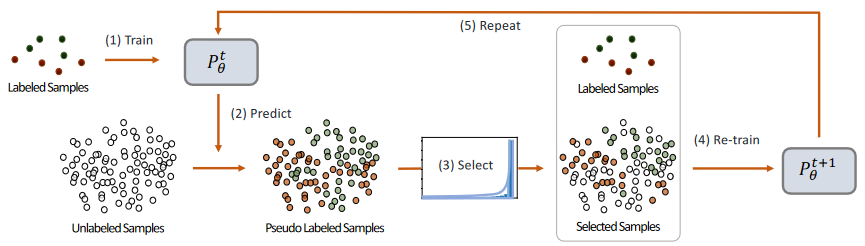
\includegraphics[width=\columnwidth]{curriculum_pseudolabelling.png}
  \caption{
    Illustration of curriculum pseudolabelling from
    \cite{cascante-bonilla2020curriculum}.
    The precise algorithm can be found in Algorithm 1 of
    \cite{cascante-bonilla2020curriculum}.
  }
  \label{fig:curr-pl}
\end{figure}

\section{Results}\label{sec:res}

\subsection{Overall Performance}\label{sec:overall-perf}

\paragraph{Experimental setup.}
We first conducted self-training experiments on a mix of model/dataset combinations,
assessing the mean test accuracy across the following data regimes: high-L, low-L
high-UL, and low-L low-UL.
(High and low refers to a proportion within $[0.25, 1]$ and $[0, 0.1]$ resp..)

Hyperparameters selected for the experiment are available at Table
\ref{tab:test_acc_hyperparams}.

\paragraph{Model performance.}
Plots for the test accuracies are available at Figure \ref{fig:ul_split_vs_l_split},
\ref{fig:test_acc_vs_ul_split_low} \& \ref{fig:test_acc_vs_ul_split_high}.
A summary of the mean and standard deviation of the test accuracies is provided in Table
\ref{tab:test_acc_summary} for easier comparison between models.

\clearpage

\begin{table}[htbp]
  \centering
  \caption{Hyperparameters selected for each dataset/model combination.}
  \label{tab:test_acc_hyperparams}
  \small
  \begin{tabular}{rccccccc}
    \toprule
    & \multicolumn{3}{c}{\normalsize\texttt{hgbt}} & \multicolumn{2}{c}{\normalsize\texttt{mlp}} & \multicolumn{2}{c}{\normalsize\texttt{random-forest}} \\
    \cmidrule(lr){2-4}
    \cmidrule(lr){5-6}
    \cmidrule(lr){7-8}
    & \texttt{lr} & \texttt{max\_depth} & \tiny\texttt{min\_samples\_leaf} & \texttt{layer\_size} & \texttt{lr} & \texttt{max\_depth} & \tiny\texttt{min\_samples\_leaf} \\
    \midrule
    \texttt{jannis} & 0.05 & - & 5 & 256 & 0.016 & - & 3 \\
    \texttt{gas-drift} & 0.025 & 2 & 5 & 192 & 0.04 & - & 1 \\
    \texttt{higgs} & 0.05 & 2 & 2 & 192 & 0.032 & - & 5 \\
    \texttt{covertype} & 0.15 & - & 3 & 192 & 0.04 & - & 1 \\
    \bottomrule
  \end{tabular}
\end{table}

\begin{table}[htbp]
  \centering
  \caption{
    Test accuracy (acc.) over five trials with mean and standard deviation.
    Within each matrix: from left to right, \texttt{ul\_split} $=$ 0 (SL), 0.25
    (high-UL); from top to bottom, \texttt{l\_split} $=$ 0.025 (low-L), 0.25 (high-L).
  }
  \label{tab:test_acc_summary}
  \begin{tabular}{rccc}
    \toprule
    & \texttt{hgbt} & \texttt{mlp} & \texttt{random-forest} \\
    \midrule
    \small\texttt{jannis}
    & \begin{minipage}[b]{0.25\columnwidth}
      \centering
      \begin{tabular}{r@{\hskip 0.1in}l}
        $62.7 \pm 6.1$ & $62.6 \pm 4.1$ \\
        $71.9 \pm 1.6$ & $71.0 \pm 2.1$ \\
      \end{tabular}
    \end{minipage}
    & \begin{minipage}[b]{0.25\columnwidth}
      \centering
      \begin{tabular}{r@{\hskip 0.1in}l}
        $64.7 \pm 4.4$ & $63.2 \pm 7.6$ \\
        $70.0 \pm 1.0$ & $70.7 \pm 0.9$ \\
      \end{tabular}
    \end{minipage}
    & \begin{minipage}[b]{0.25\columnwidth}
      \centering
      \begin{tabular}{r@{\hskip 0.1in}l}
        $66.1 \pm 3.9$ & $62.1 \pm 3.8$ \\
        $71.6 \pm 1.6$ & $69.8 \pm 1.9$ \\
      \end{tabular}
    \end{minipage} \\ \addlinespace
    \small\texttt{gas-drift}
    & \begin{minipage}[b]{0.25\columnwidth}
      \centering
      \begin{tabular}{r@{\hskip 0.1in}l}
        $65.3 \pm 3.7$ & $64.5 \pm 2.2$ \\
        $94.7 \pm 0.4$ & $95.0 \pm 0.7$ \\
      \end{tabular}
    \end{minipage}
    & \begin{minipage}[b]{0.25\columnwidth}
      \centering
      \begin{tabular}{r@{\hskip 0.1in}l}
        $76.1 \pm 2.9$ & $66.0 \pm 7.0$ \\
        $97.0 \pm 0.1$ & $97.2 \pm 0.4$ \\
      \end{tabular}
    \end{minipage}
    & \begin{minipage}[b]{0.25\columnwidth}
      \centering
      \begin{tabular}{r@{\hskip 0.1in}l}
        $67.5 \pm 3.4$ & $64.4 \pm 5.3$ \\
        $93.1 \pm 0.8$ & $92.9 \pm 1.3$ \\
      \end{tabular}
    \end{minipage} \\ \addlinespace
    \small\texttt{higgs}
    & \begin{minipage}[b]{0.25\columnwidth}
      \centering
      \begin{tabular}{r@{\hskip 0.1in}l}
        $54.8 \pm 2.1$ & $53.0 \pm 1.8$ \\
        $65.6 \pm 1.7$ & $64.0 \pm 1.2$ \\
      \end{tabular}
    \end{minipage}
    & \begin{minipage}[b]{0.25\columnwidth}
      \centering
      \begin{tabular}{r@{\hskip 0.1in}l}
        $52.1 \pm 2.7$ & $51.5 \pm 2.3$ \\
        $54.9 \pm 2.9$ & $53.3 \pm 3.3$ \\
      \end{tabular}
    \end{minipage}
    & \begin{minipage}[b]{0.25\columnwidth}
      \centering
      \begin{tabular}{r@{\hskip 0.1in}l}
        $53.8 \pm 2.7$ & $51.5 \pm 3.2$ \\
        $65.8 \pm 0.9$ & $62.5 \pm 1.4$ \\
      \end{tabular}
    \end{minipage} \\ \addlinespace
    \small\texttt{covertype}
    & \begin{minipage}[b]{0.25\columnwidth}
      \centering
      \begin{tabular}{r@{\hskip 0.1in}l}
        $52.6 \pm 2.4$ & $52.0 \pm 3.8$ \\
        $68.1 \pm 0.8$ & $67.4 \pm 1.2$ \\
      \end{tabular}
    \end{minipage}
    & \begin{minipage}[b]{0.25\columnwidth}
      \centering
      \begin{tabular}{r@{\hskip 0.1in}l}
        $49.8 \pm 2.4$ & $42.2 \pm 6.9$ \\
        $59.7 \pm 6.2$ & $62.5 \pm 1.3$ \\
      \end{tabular}
    \end{minipage}
    & \begin{minipage}[b]{0.25\columnwidth}
      \centering
      \begin{tabular}{r@{\hskip 0.1in}l}
        $52.8 \pm 2.6$ & $45.0 \pm 2.6$ \\
        $69.3 \pm 1.3$ & $68.4 \pm 1.2$ \\
      \end{tabular}
    \end{minipage} \\
    \bottomrule
  \end{tabular}
\end{table}

\begin{figure}[htbp]
  \centering
  \includesvg[width=\columnwidth]{test_accs/jannis_ul_split_vs_l_split.svg}
  \includesvg[width=\columnwidth]{test_accs/gas-drift-different-concentrations_ul_split_vs_l_split.svg}
  \includesvg[width=\columnwidth]{test_accs/higgs_ul_split_vs_l_split.svg}
  \includesvg[width=\columnwidth]{test_accs/covertype_ul_split_vs_l_split.svg}
  \caption{Test accuracy (acc.) across different splits.}
  \label{fig:ul_split_vs_l_split}
\end{figure}

\begin{figure}[htbp]
  \centering
  \includesvg[width=\columnwidth]{test_accs/jannis_test_acc_vs_ul_split_low.svg}
  \includesvg[width=\columnwidth]{test_accs/gas-drift-different-concentrations_test_acc_vs_ul_split_low.svg}
  \includesvg[width=\columnwidth]{test_accs/higgs_test_acc_vs_ul_split_low.svg}
  \includesvg[width=\columnwidth]{test_accs/covertype_test_acc_vs_ul_split_low.svg}
  \caption{
    Test accuracy (acc.) across different splits in the low unlabelled (UL) data regime.
  }
  \label{fig:test_acc_vs_ul_split_low}
\end{figure}

\begin{figure}[htbp]
  \centering
  \includesvg[width=\columnwidth]{test_accs/jannis_test_acc_vs_ul_split_high.svg}
  \includesvg[width=\columnwidth]{test_accs/gas-drift-different-concentrations_test_acc_vs_ul_split_high.svg}
  \includesvg[width=\columnwidth]{test_accs/higgs_test_acc_vs_ul_split_high.svg}
  \includesvg[width=\columnwidth]{test_accs/covertype_test_acc_vs_ul_split_high.svg}
  \caption{
    Test accuracy (acc.) across different splits in the high unlabelled (UL) data regime.
  }
  \label{fig:test_acc_vs_ul_split_high}
\end{figure}

\paragraph{Variability of MLP performance.}
While tree-based models typically dominate in performance across data regimes, we find
that MLPs are subject to greater variability in performance across tabular datasets,
with MLPs performing significantly better on \texttt{gas-drift-different-concentrations}
and worse on \texttt{covertype} (see Figure \ref{fig:ul_split_vs_l_split}).

\paragraph{Curriculum self-training wo/ input consistency regularisation vs supervised
learning.}
Generally, we find that curriculum self-training without input consistency
regularisation does not offer much benefit over supervised learning.\footnote{%
  The theoretical results of \cite{wei2022theoretical} apply only when input consistency
  regularisation is applied in training.
}
Notably, in the low-L data regime, incorporating high-UL data can occasionally lead to
trials with very poor performance, although self-training produces comparable results
most of the time (see top row of matrices in Table \ref{tab:test_acc_summary}, which
often has high standard deviations at the top right).
We study this phenomenon in more detail under Section \ref{sec:det_anal_jannis_mlp}.

\clearpage
\paragraph{Evolution of models in curriculum self-training.}
Lastly, we attach interactive parallel coordinate plots showing how validation accuracy
changes over pseudolabelling iterations.
For ease of viewing, it is recommended to select specific regions of the graph, e.g. to
see how all experiments performed on a single split, you can select
\texttt{args.seed=0}, \texttt{split.l\_split=0.025}, \texttt{split.ul\_split=0.25}.
{
  \small
  \begin{enumerate}
    \item \texttt{jannis}: \begin{enumerate}
      \item \texttt{hgbt}: \url{https://api.wandb.ai/links/wei2912/52kfpcnd}
      \item \texttt{mlp}: \url{https://wandb.ai/wei2912/ethz-ssl-tabular_jannis/reports/-20230804-Parallel-Coordinate-Plots-mlp---Vmlldzo1MDU0ODM2?accessToken=nqsx9rdqqeejs3fzdnf1x1oo1n8wlfqhe5yx4s6i4oaiz6djm742t2gqactp66ps}
      \item \texttt{random-forest}: \url{https://wandb.ai/wei2912/ethz-ssl-tabular_jannis/reports/-20230804-Parallel-Coordinate-Plots-random-forest---Vmlldzo1MDU0ODQy?accessToken=nywqnqx9cwx1sib3361au2ynljiba3tgj9d9d5064rejzrcn8nkoypfitvrbhs1x}
    \end{enumerate}
    \item \texttt{gas-drift}: \begin{enumerate}
      \item \texttt{hgbt}: \url{https://api.wandb.ai/links/wei2912/5ljhsi70}
      \item \texttt{mlp}: \url{https://api.wandb.ai/links/wei2912/mcdsxevg}
      \item \texttt{random-forest}: \url{https://api.wandb.ai/links/wei2912/fld4y2bj}
    \end{enumerate}
    \item \texttt{higgs}: \begin{enumerate}
      \item \texttt{hgbt}: \url{https://wandb.ai/wei2912/ethz-ssl-tabular_higgs/reports/-20230804-Parallel-Coordinate-Plots-hgbt---Vmlldzo1MDU0ODQ5?accessToken=mmunbdr38oqrjxy8cx33va19xfflkdo7d95rxmvcnhf4uw32gdrec6prmj5pj3ny}
      \item \texttt{mlp}: \url{https://wandb.ai/wei2912/ethz-ssl-tabular_higgs/reports/-20230804-Parallel-Coordinate-Plots-mlp---Vmlldzo1MDU0OTgx?accessToken=0klorbel8nf1shcw6cu2djl6hb6cmbq3sikh79n3qzw788tjwhkifo6cw24lcwn7}
      \item \texttt{random-forest}: \url{https://api.wandb.ai/links/wei2912/kcp3hgny}
    \end{enumerate}
    \item \texttt{covertype}: \begin{enumerate}
      \item \texttt{hgbt}: \url{https://wandb.ai/wei2912/ethz-ssl-tabular_covertype/reports/-20230804-Parallel-Coordinate-Plots-hgbt---Vmlldzo1MDU0Njkz?accessToken=8uejk4mwds8zbghhx799fejblqz1o3z3dhkz6o48jfk6hcncsx1et7n264s5jatm}
      \item \texttt{mlp}: \url{https://wandb.ai/wei2912/ethz-ssl-tabular_covertype/reports/-20230804-Parallel-Coordinate-Plots-mlp---Vmlldzo1MDU0Njg1?accessToken=lyt6ngnatcslorp5d02biv61eo4mso0t34j0bea6ledq5787of3ygnjok0vy03j4}
      \item \texttt{random-forest}: \url{https://wandb.ai/wei2912/ethz-ssl-tabular_covertype/reports/-20230804-Parallel-Coordinate-Plots-random-forest---Vmlldzo1MDU0NTA5?accessToken=z1ac8yvyfv3m8i24711z8wmpae2h09jo0xsy2wrpurp3i3h6ute802kh80gg9s4y}
    \end{enumerate}
  \end{enumerate}
}

\clearpage
\subsection{Detailed Analysis of \texttt{jannis/mlp} in low-L regime}
\label{sec:det_anal_jannis_mlp}

\paragraph{Collapsing of models in curriculum self-training.}
In Figure \ref{fig:par_coords_jannis_mlp}, we observed that for \texttt{l\_split=0.025}
(low-L), some runs perform at reasonable accuracies while a few runs (see dark blue
curves) experienced a collapse in test accuracies.

Curiously, such runs often have an initial validation accuracy
(\texttt{run.initial.val.acc} with the model trained on only the L dataset) comparable
to that of other runs ($> 60\%$), but after a few pseudolabelling iterations (trained on
80-100\% of the pseudolabelled UL dataset), collapse to $\sim 50\%$ validation accuracy
(see \texttt{run.pl\_iter\{0..4\}.val.acc}).
As \texttt{jannis} is a binary classification problem, this effectively means the models
are as good as random.

This phenomenon appears to occur more frequently in low-L high-UL data regimes, as
compared to low-L low-UL, although more experiments are required to verify this.

\begin{figure}[htbp]
  \centering
  \includegraphics[width=\columnwidth]{par_coords_jannis_mlp.png}
  \caption{Parallel coordinate plot for \texttt{jannis}/\texttt{mlp} with
  \texttt{l\_split=0.025} (low-L), available at
  {\small\url{https://wandb.ai/wei2912/ethz-ssl-tabular_jannis/reports/-20230804-Parallel-Coordinate-Plots-mlp---Vmlldzo1MDU0ODM2?accessToken=nqsx9rdqqeejs3fzdnf1x1oo1n8wlfqhe5yx4s6i4oaiz6djm742t2gqactp66ps}}.}
  \label{fig:par_coords_jannis_mlp}
\end{figure}

\afterpage{\clearpage}
\paragraph{Dataset label noise.}
We conducted some preliminary experiments to examine if the reason for the collapse in
validation accuracy is solely due to random dataset label noise:
\begin{enumerate}
  \item Setting \texttt{seed=5}, \texttt{l\_split=0.05}, \texttt{ul\_split=0.75} (such
  that all experiments are provided the same dataset split), we identified a single
  trial which collapsed to 54.4\% validation accuracy and computed the dataset label
  accuracy (\texttt{l\_pl\_acc}) of 64.1\% on the 5th and final pseudolabelling
  iteration (\texttt{pl\_iter4}), which pseudolabels the entire UL dataset.
  This pseudolabelled dataset is used to train the final model from scratch.
  \item Afterwards, we simulated 40 trials of a ``fake'' self-training method, which
  randomly corrupts the ground-truth labels of the entire UL dataset to achieve a
  similar dataset label accuracy, before training a new model on this dataset.
\end{enumerate}
In Figure \ref{fig:par_coords_jannis_mlp_simul_noise}, we found that all runs of the
``fake'' self-training method achieved $> 59\%$ validation accuracy, significantly
higher than that of the single trial at 54.4\%.
This suggests that the label noise generated by pseudolabelling may have stronger
adversarial effects than uniform label noise.
Consequently, curriculum self-training in the low-L high-UL data regime might require
modifications to stabilise the training process.
Plots with more runs are available in Section \ref{sec:icr_jannis_mlp}.

\begin{figure}[htbp]
  \centering
  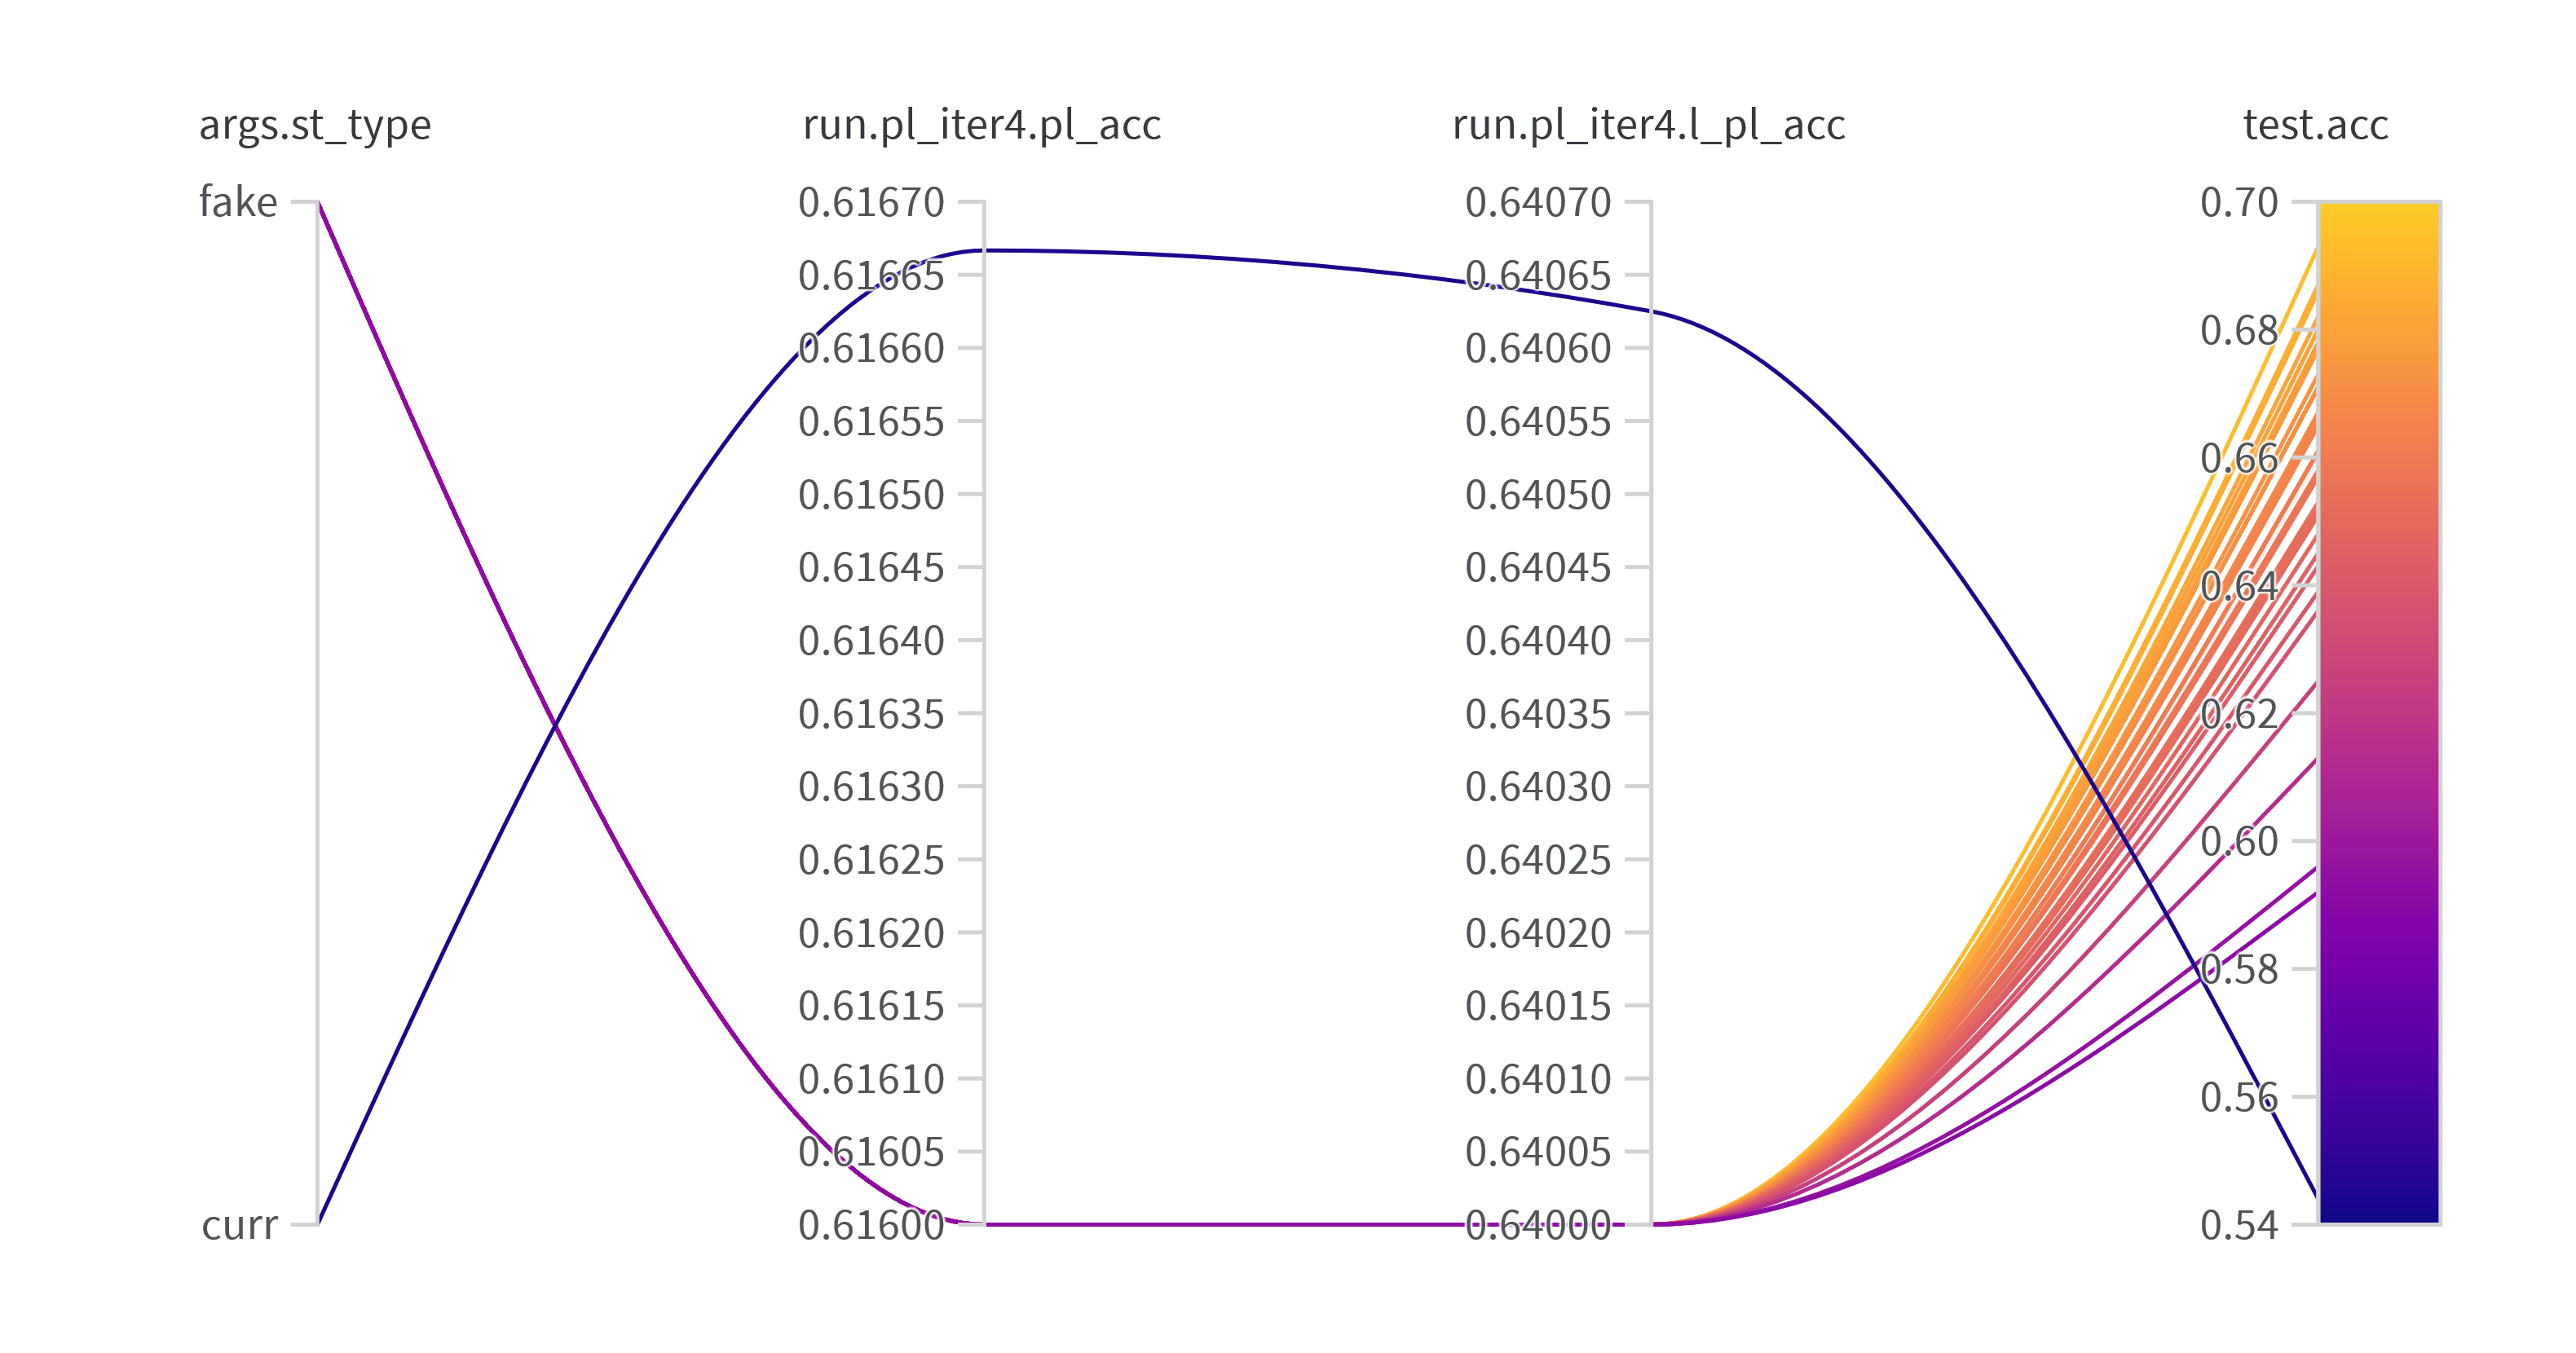
\includegraphics[width=\columnwidth]{par_coords_jannis_mlp_simul_noise.png}
  \caption{
    Parallel coordinate plot for \texttt{jannis}/\texttt{mlp} with
    \texttt{l\_split=0.05} and \texttt{ul\_split=0.75} over the same dataset split.
    \texttt{pl\_acc} and \texttt{l\_pl\_acc} refer to the label accuracy of the
    pseudolaelled (PL) dataset and the entire training dataset (L \& PL) resp..
  }
  \label{fig:par_coords_jannis_mlp_simul_noise}
\end{figure}

\subsection{Input Consistency Regularisation with \texttt{jannis/mlp}}
\label{sec:icr_jannis_mlp}

\paragraph{Input consistency regularisation.}
Input consistency regularisation techniques, such as Virtual Adversarial Training (VAT)
\cite{miyato2018virtual} and Unsupervised Data Augmentation (UDA)
\cite{xie2020unsupervised}, encourage models to learn representations such that data
augmentation transformations on samples preserve their original predicted labels.
The former was used to experimentally demonstrate the results of
\textcite{wei2022theoretical} and show that incorrect pseudolabels can be denoised by
deep models trained with input consistency regularisation.

\paragraph{Challenges on tabular data.}
VAT relies on adversarial perturbations, while UDA can be used with more general data
augmentation techniques (i.e. rotation/flipping for images).
As such, we picked UDA for its simplicity of implementation.
However, unlike for visual modality, there is no commonly used set of data augmentation
transformations proposed for tabular data.\footnote{%
  Simply adding random perturbations to (normalised) features may no longer preserve
  labels, since optimal decision boundaries for tabular datasets may not be smooth (see
  Appendix A.4 of \cite{grinsztajn2022why}).
  SCARF-style corruptions, which we employ in our work, were also shown to be more
  effective to other common alternatives \cite{bahri2022scarf}.
}

\paragraph{UDA with SCARF-style corruptions.}
Following SCARF \cite{bahri2022scarf}, a self-supervised contrastive learning method for
tabular data, we perform data augmentations through feature corruptions.
For each sample in a batch, we choose 60\% of features to replace with randomly sampled
values from the features' respective empirical marginal distribution (based on the
entire L/UL dataset).

Since we employ UDA, only UL samples are augmented, with the following loss term%
\footnote{%
  While this loss term can be weighed by a constant factor $\lambda$, we follow
  \cite{xie2020unsupervised} in setting $\lambda = 1$ for simplicity.
} added to the standard cross-entropy loss objective \cite{xie2020unsupervised}:
\begin{equation}
  \mathbb{E}_{x \sim p_\text{UL}}\,
  \mathbb{E}_{\hat{x} \sim q(\hat{x} \mid x)}\,
  \CE{p_{\tilde{\theta}}(y \mid x)}{p_\theta(y \mid \hat{x})},
\end{equation} where:
\begin{itemize}
  \item $p_\text{UL}$ is the distribution of unlabelled samples;
  \item $q(\hat{x} \mid x)$ is the distribution of samples after transforming the sample
  $x$;
  \item $\CE{\cdot}{\cdot}$ is the cross-entropy loss;
  \item $p_\theta(y \mid x)$ is the output distribution of the model with parameters
  $\theta$; and
  \item $\tilde{\theta}$ is a fixed copy of the current parameters $\theta$, to prevent
  the gradient from propagating through $\tilde{\theta}$.
\end{itemize}
The original UL samples $x$ and corrupted UL samples $\hat{x}$ are randomly drawn on
every iteration to compute this loss term.
Effectively, this encourages the model to predict the same labels on any input and their
corrupted versions, gaining information on the input distribution by exploiting the
large size of the UL dataset.

\paragraph{Model performance.}
For \texttt{jannis/mlp}, we tested four different training methods on \texttt{ul\_split}
$=$ 0 (SL), 0.25 (high-UL) and \texttt{l\_split} $=$ 0.025 (low-L), 0.25 (high-L):
\begin{itemize}
  \item \texttt{none}: SL model.
  \item \texttt{uda}: SL model with UDA applied.
  \item \texttt{curr}: Curriculum self-training on SL model without input consistency
  regularisation.
  \item \texttt{curr-uda}: Curriculum self-training on SL model with UDA applied.
\end{itemize}
We used a total of 10 splits (\texttt{seed} $=$ 0..9) with 5 trials on each split,
leading to a total of 50 runs.
Plots are available in Figure \ref{fig:par_coords_jannis_mlp_icr_l_split_low},
\ref{fig:par_coords_jannis_mlp_icr_l_split_high}.

\begin{figure}[htbp]
  \centering
  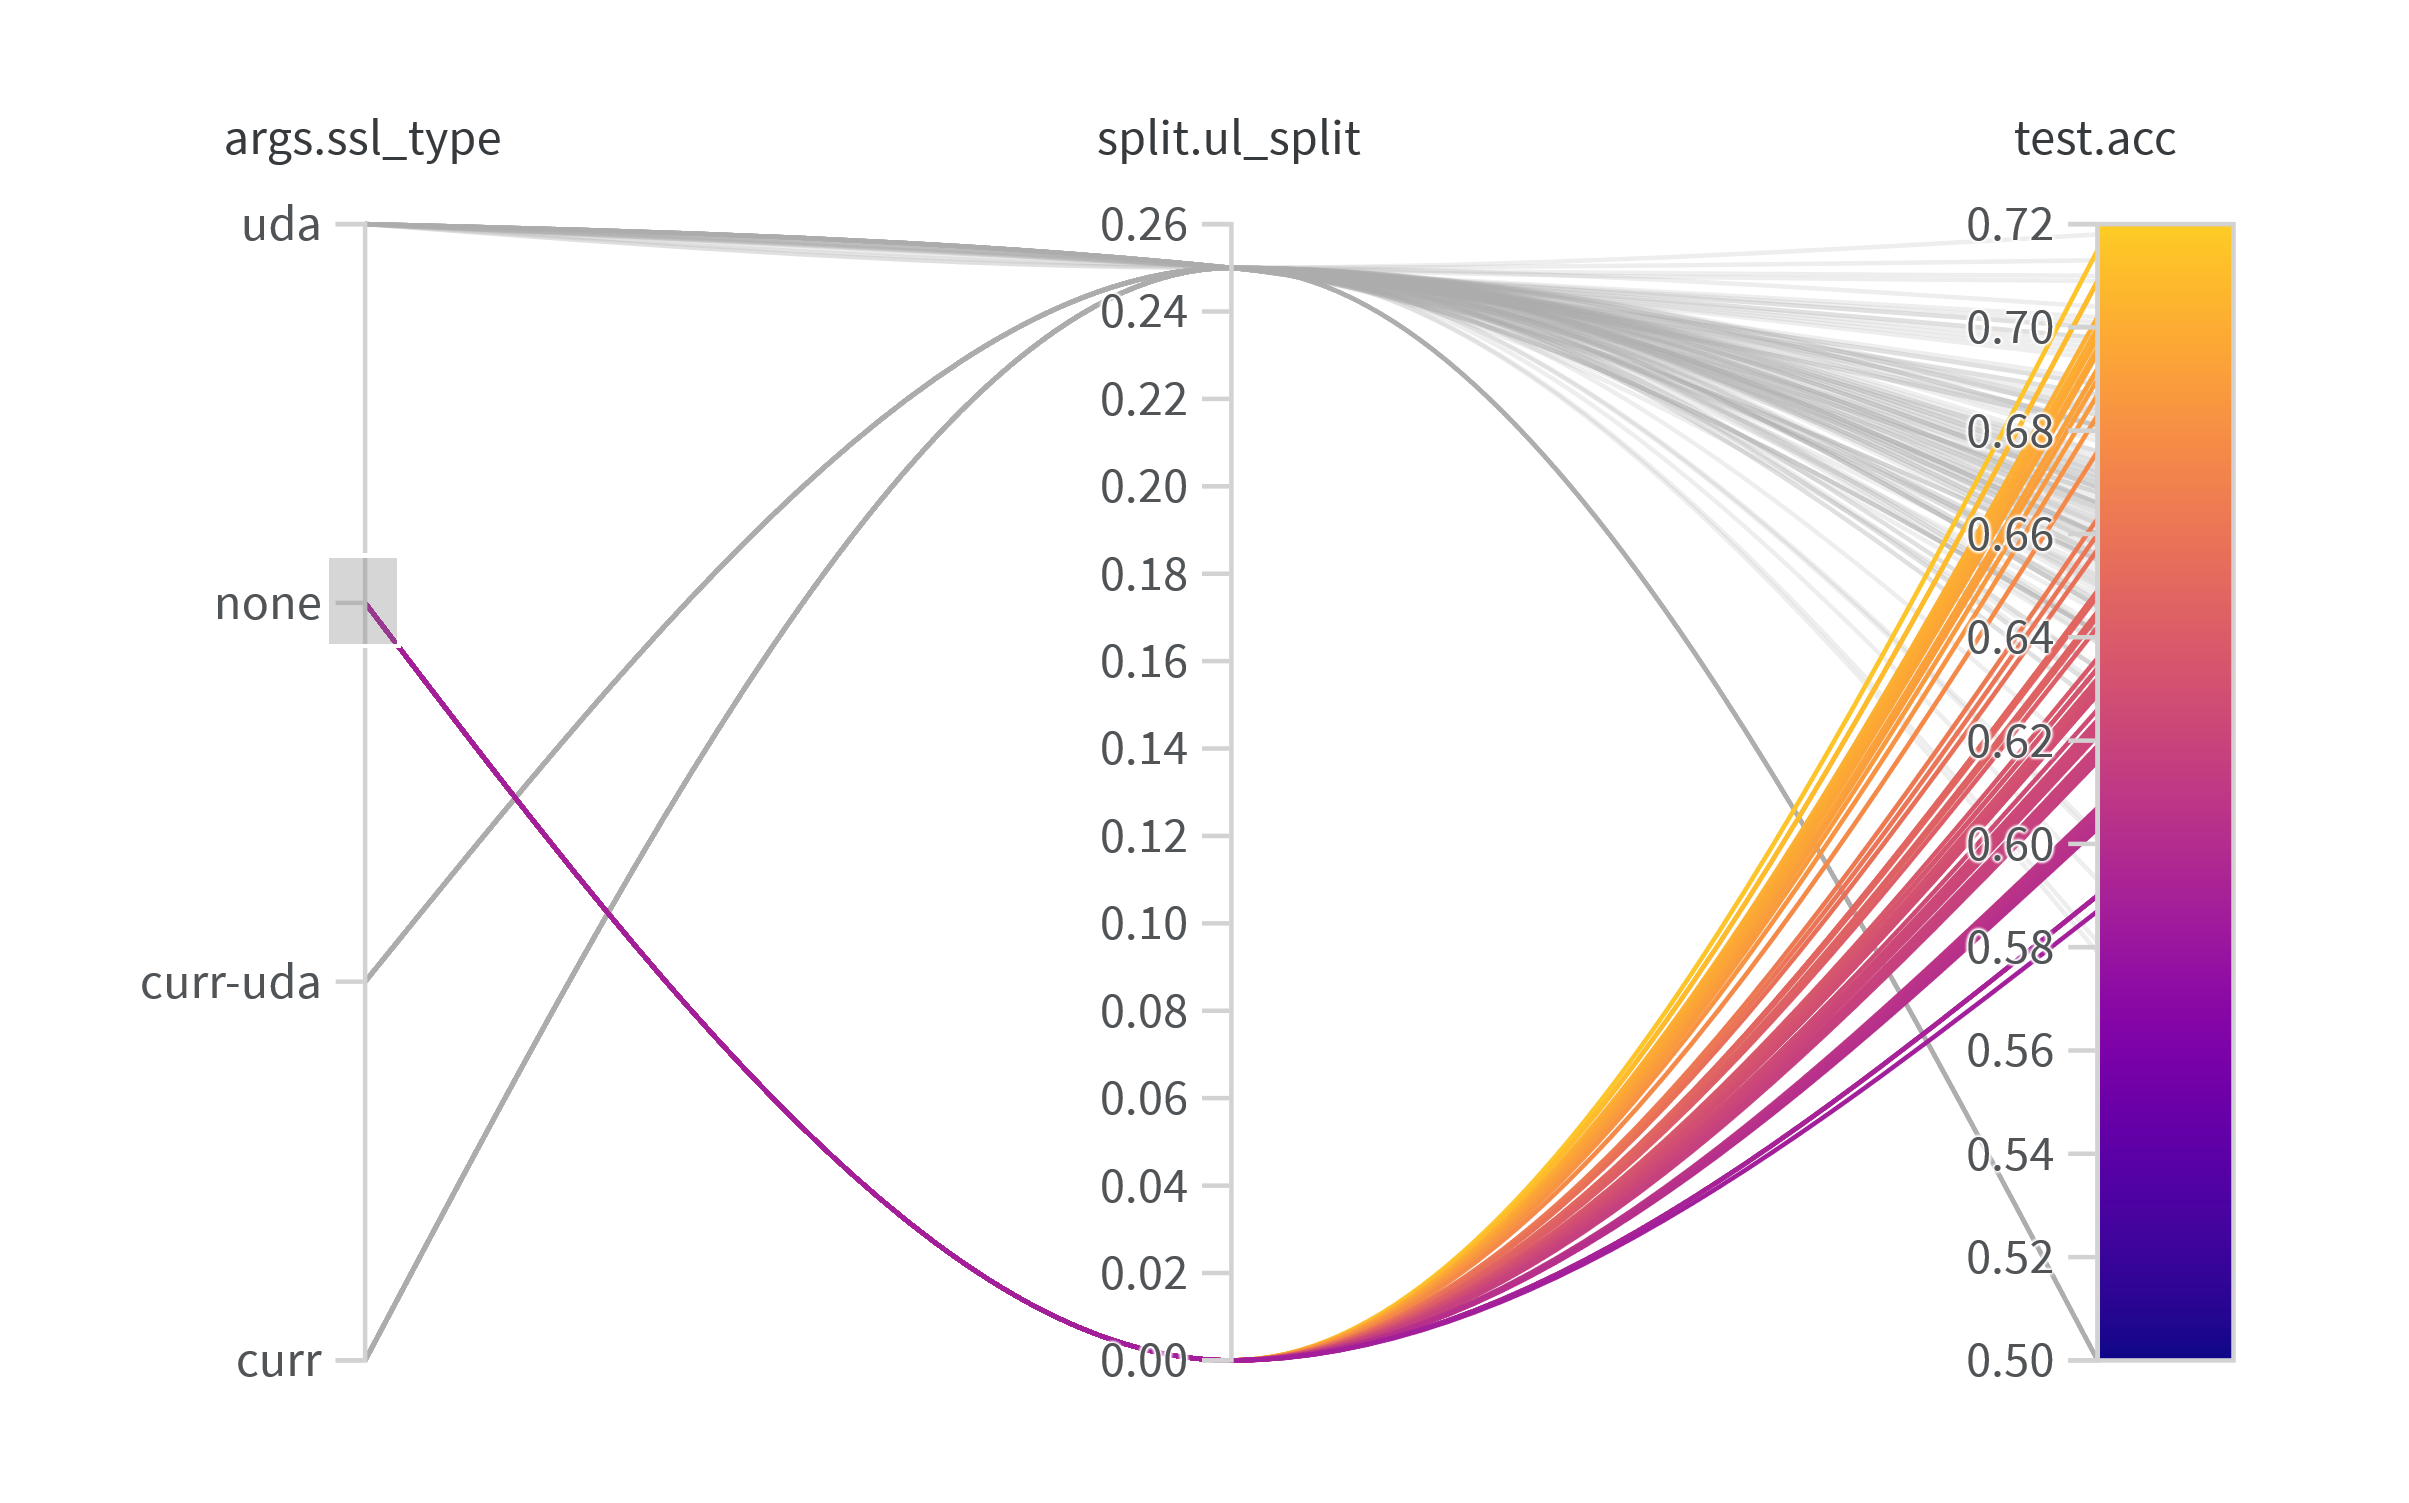
\includegraphics[width=0.48\columnwidth]{par_coords_jannis_mlp_icr_l_split_low_none.png}
  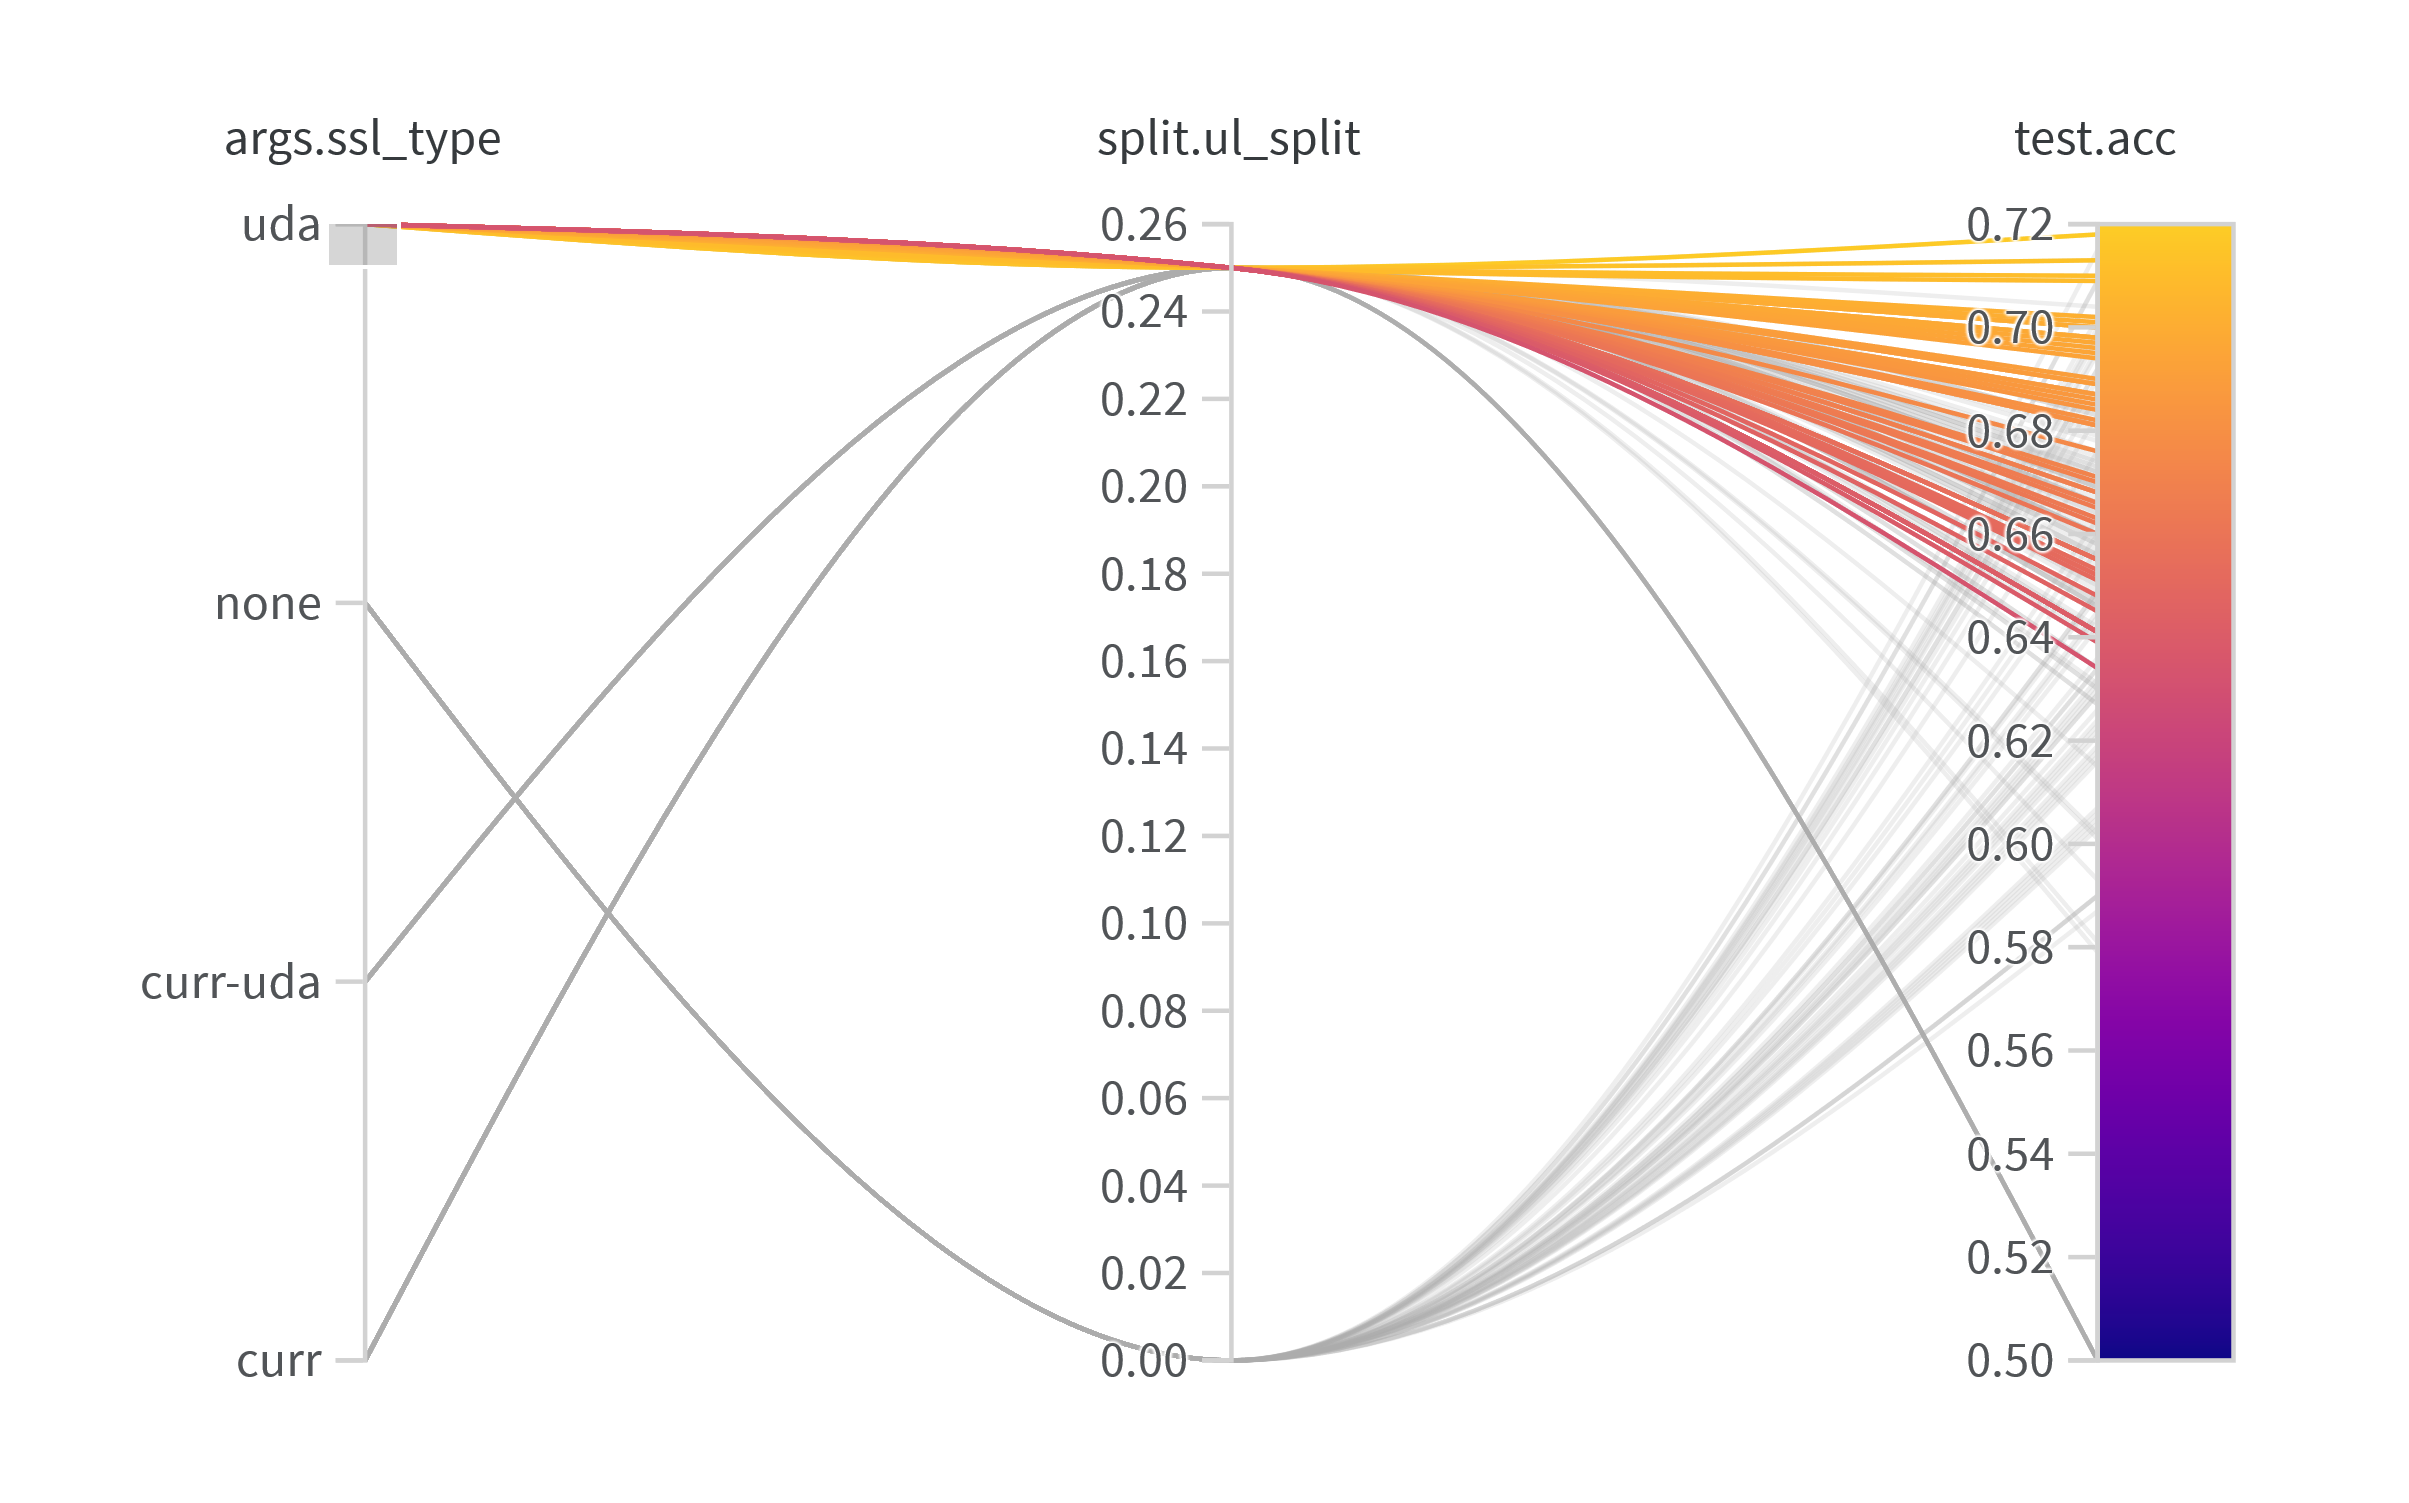
\includegraphics[width=0.48\columnwidth]{par_coords_jannis_mlp_icr_l_split_low_uda.png}
  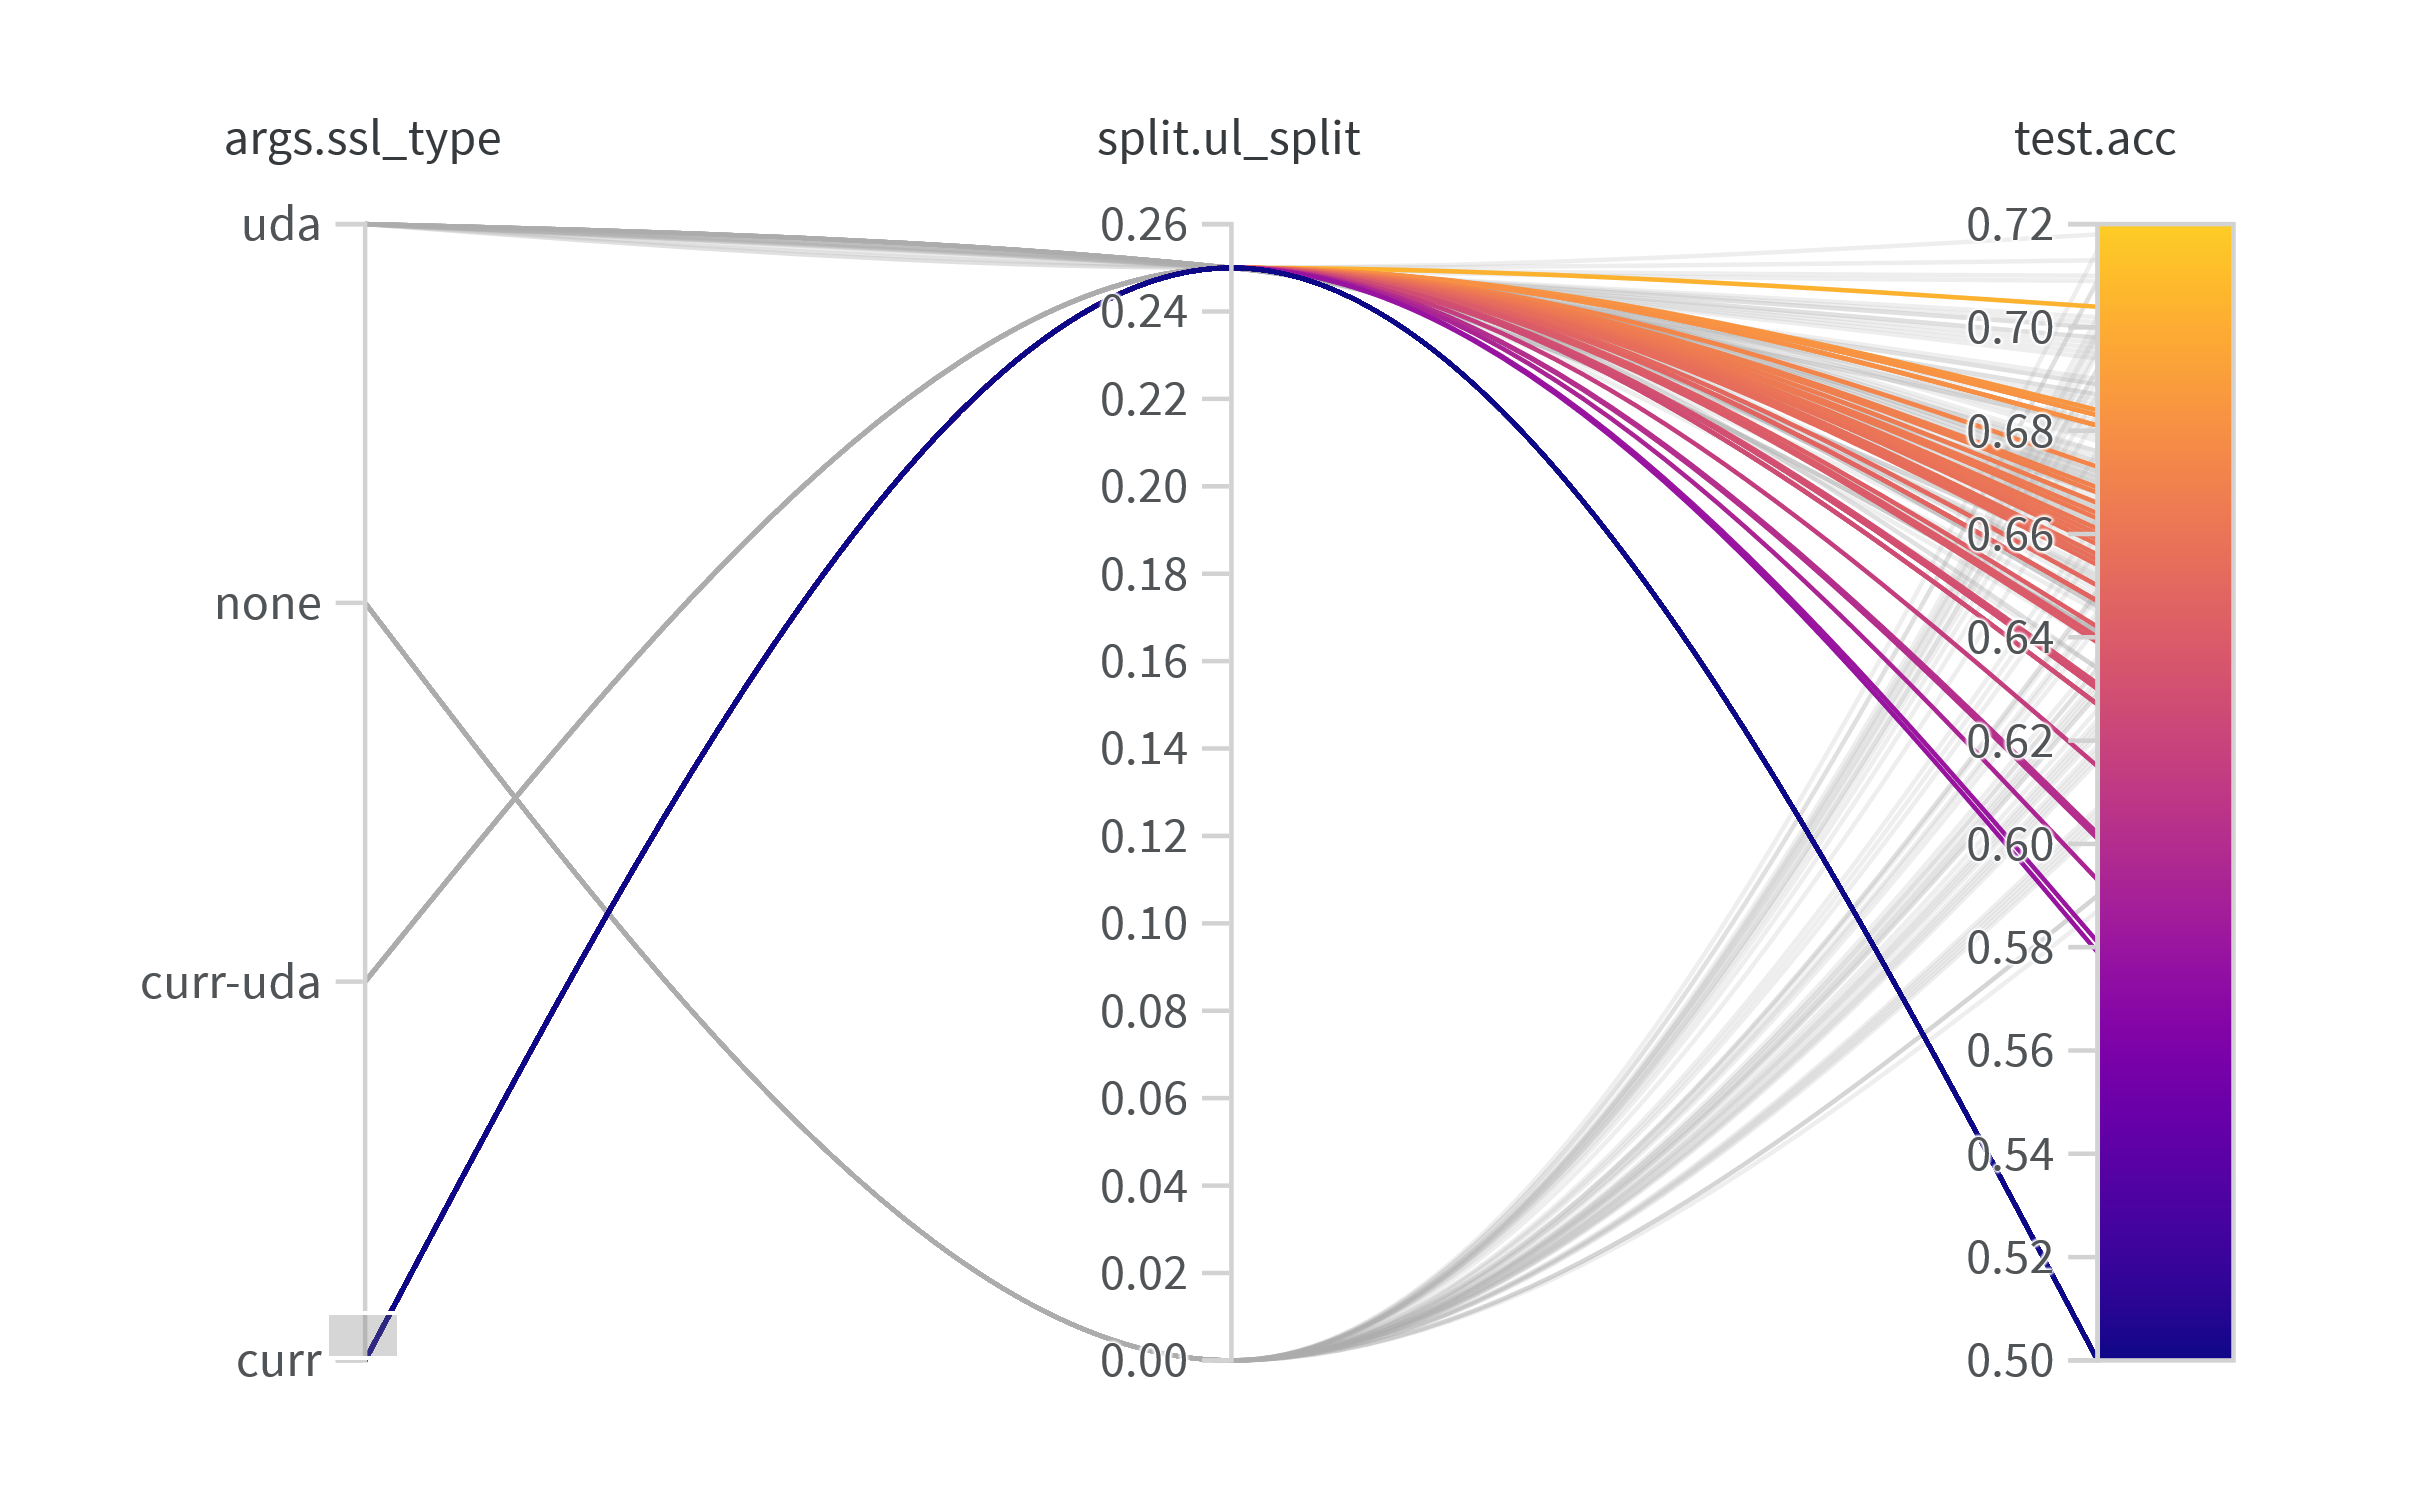
\includegraphics[width=0.48\columnwidth]{par_coords_jannis_mlp_icr_l_split_low_curr.png}
  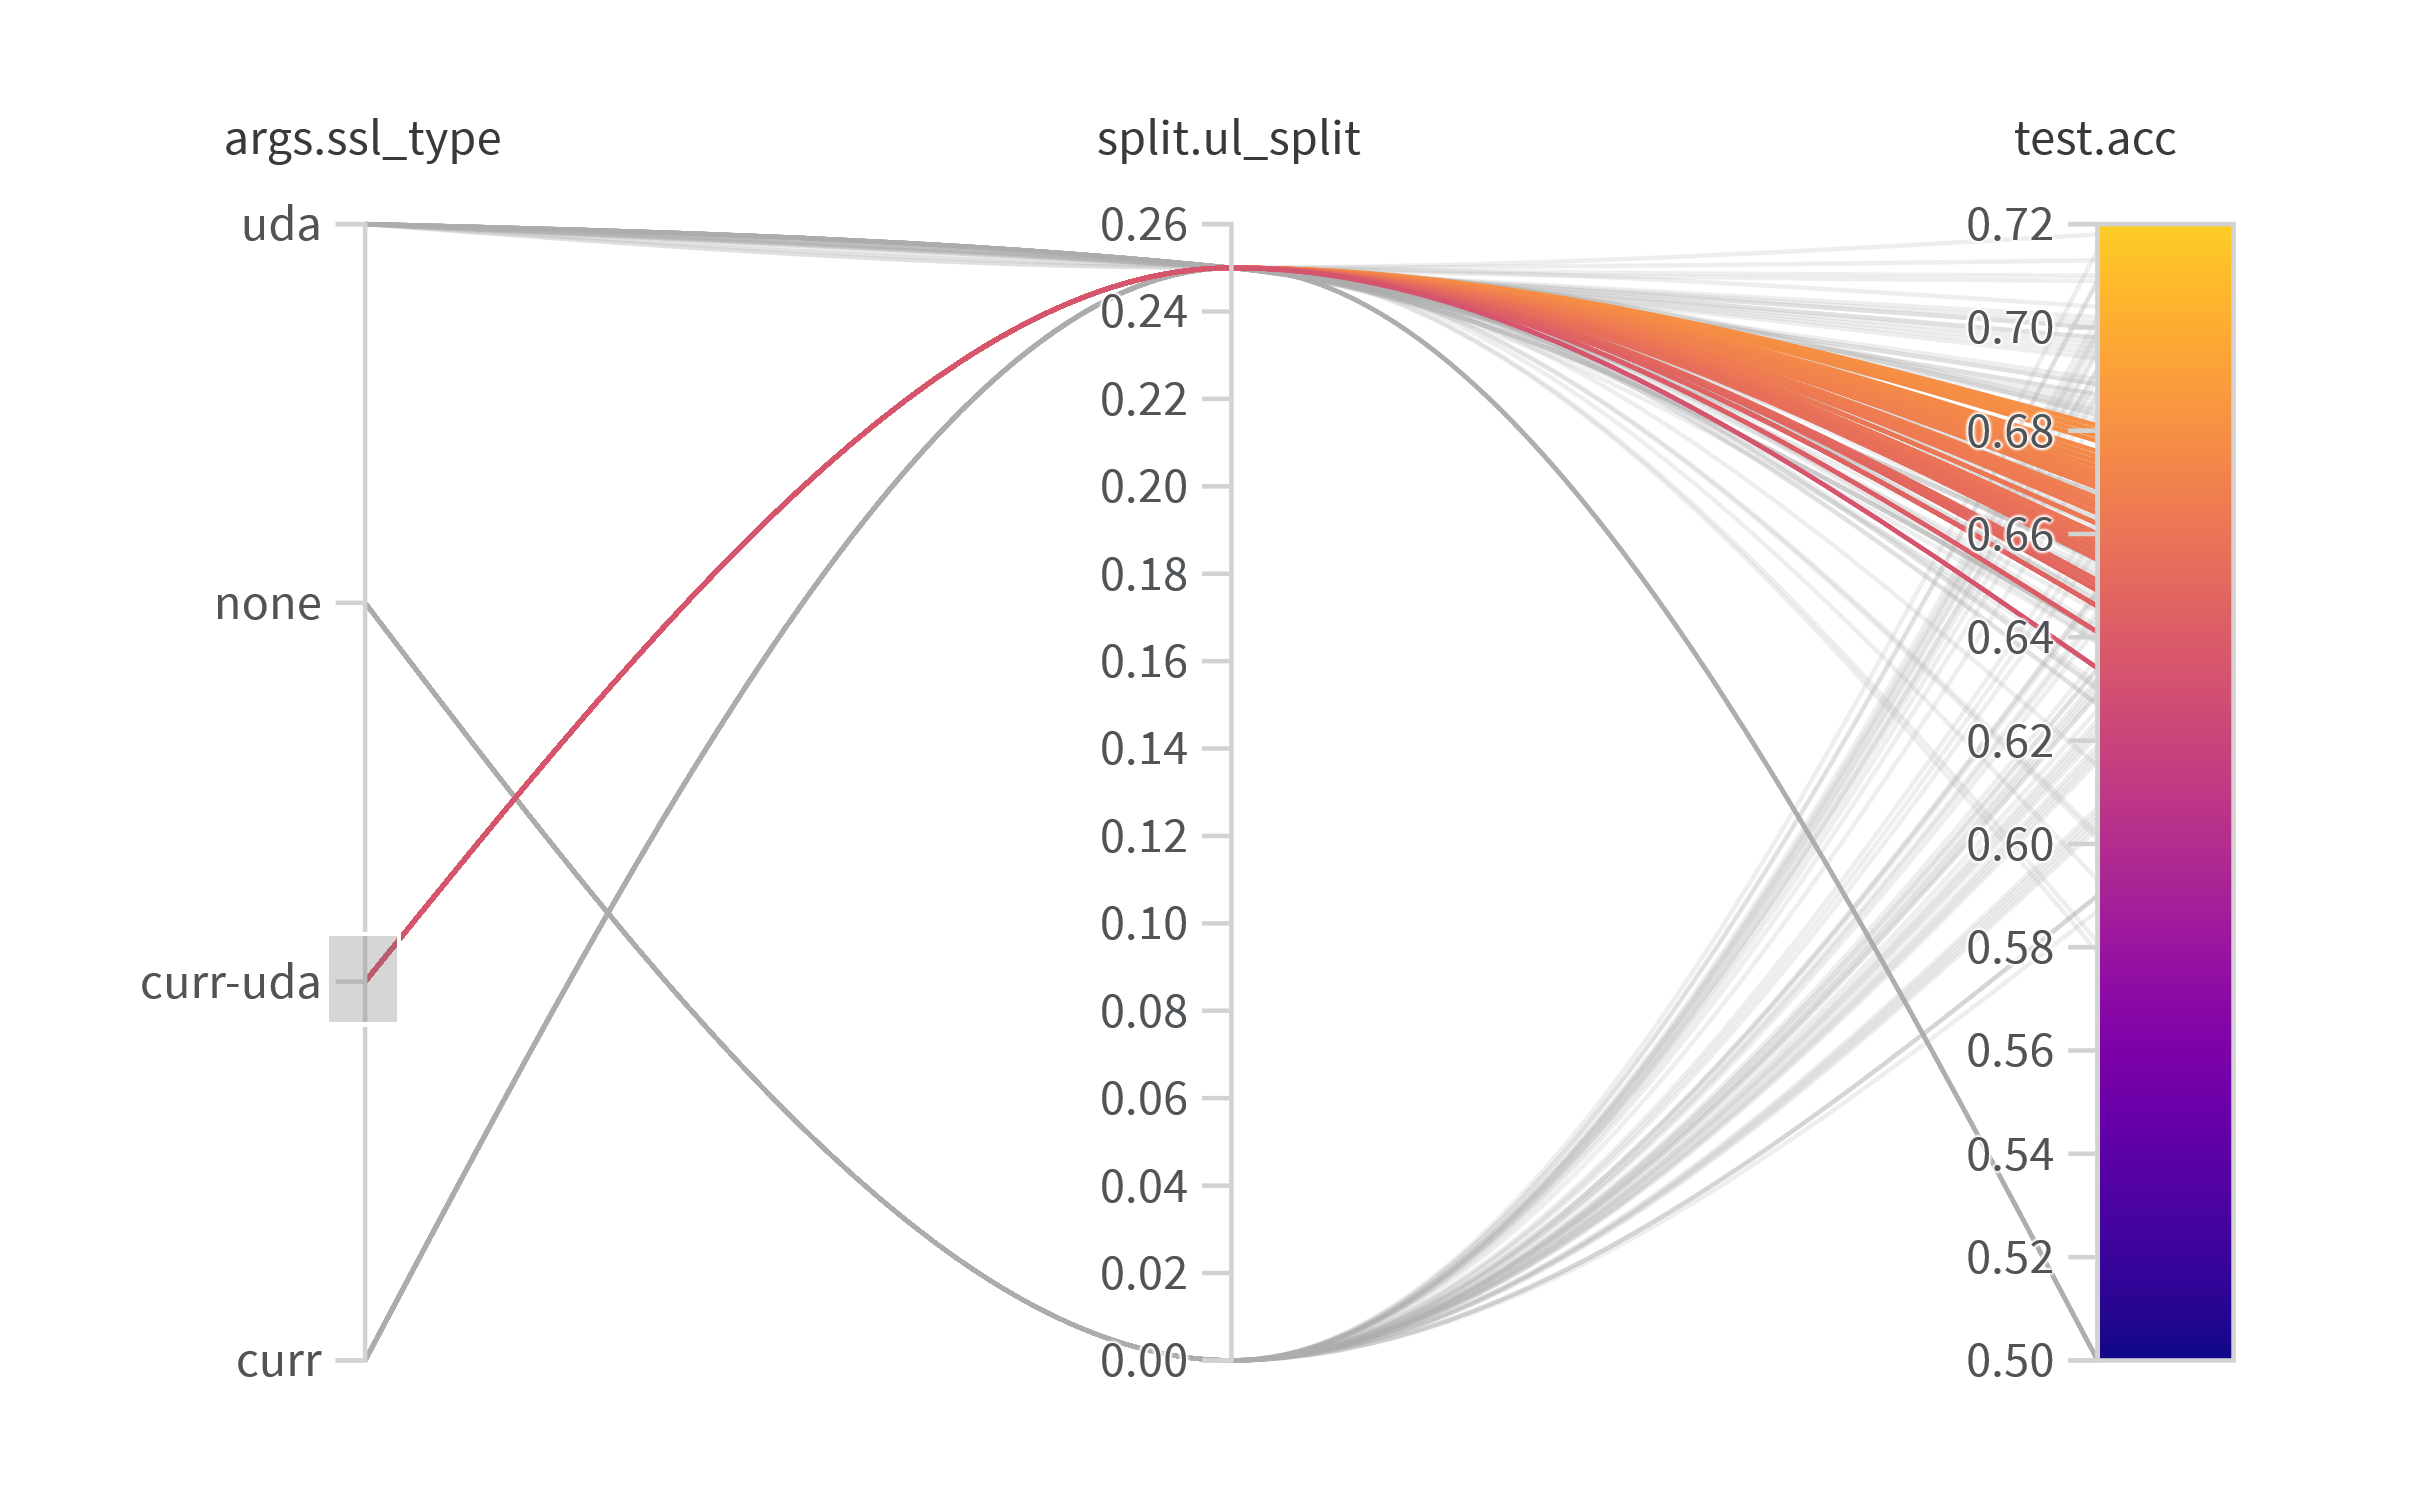
\includegraphics[width=0.48\columnwidth]{par_coords_jannis_mlp_icr_l_split_low_curr-uda.png}
  \caption{
    Parallel coordinate plots for \texttt{jannis}/\texttt{mlp} with
    \texttt{l\_split=0.025} (low-L).
    From top left to top right, \texttt{none} and \texttt{uda}; from bottom left to
    bottom right, \texttt{curr} and \texttt{curr-uda}.
    More interactive plots are available at
    {\small\url{https://wandb.ai/wei2912/ethz-ssl-tabular_jannis/reports/-20230828-Parallel-Coordinate-Plots-mlp-l_split-0-025---Vmlldzo1MjUxNTIy?accessToken=ck5tv0ze21f0499gc2ple2axkyjofxc0w7x74uxrccr78aqwdqx69uqiyq93avkn}}.
  }
  \label{fig:par_coords_jannis_mlp_icr_l_split_low}
\end{figure}

\begin{figure}[htbp]
  \centering
  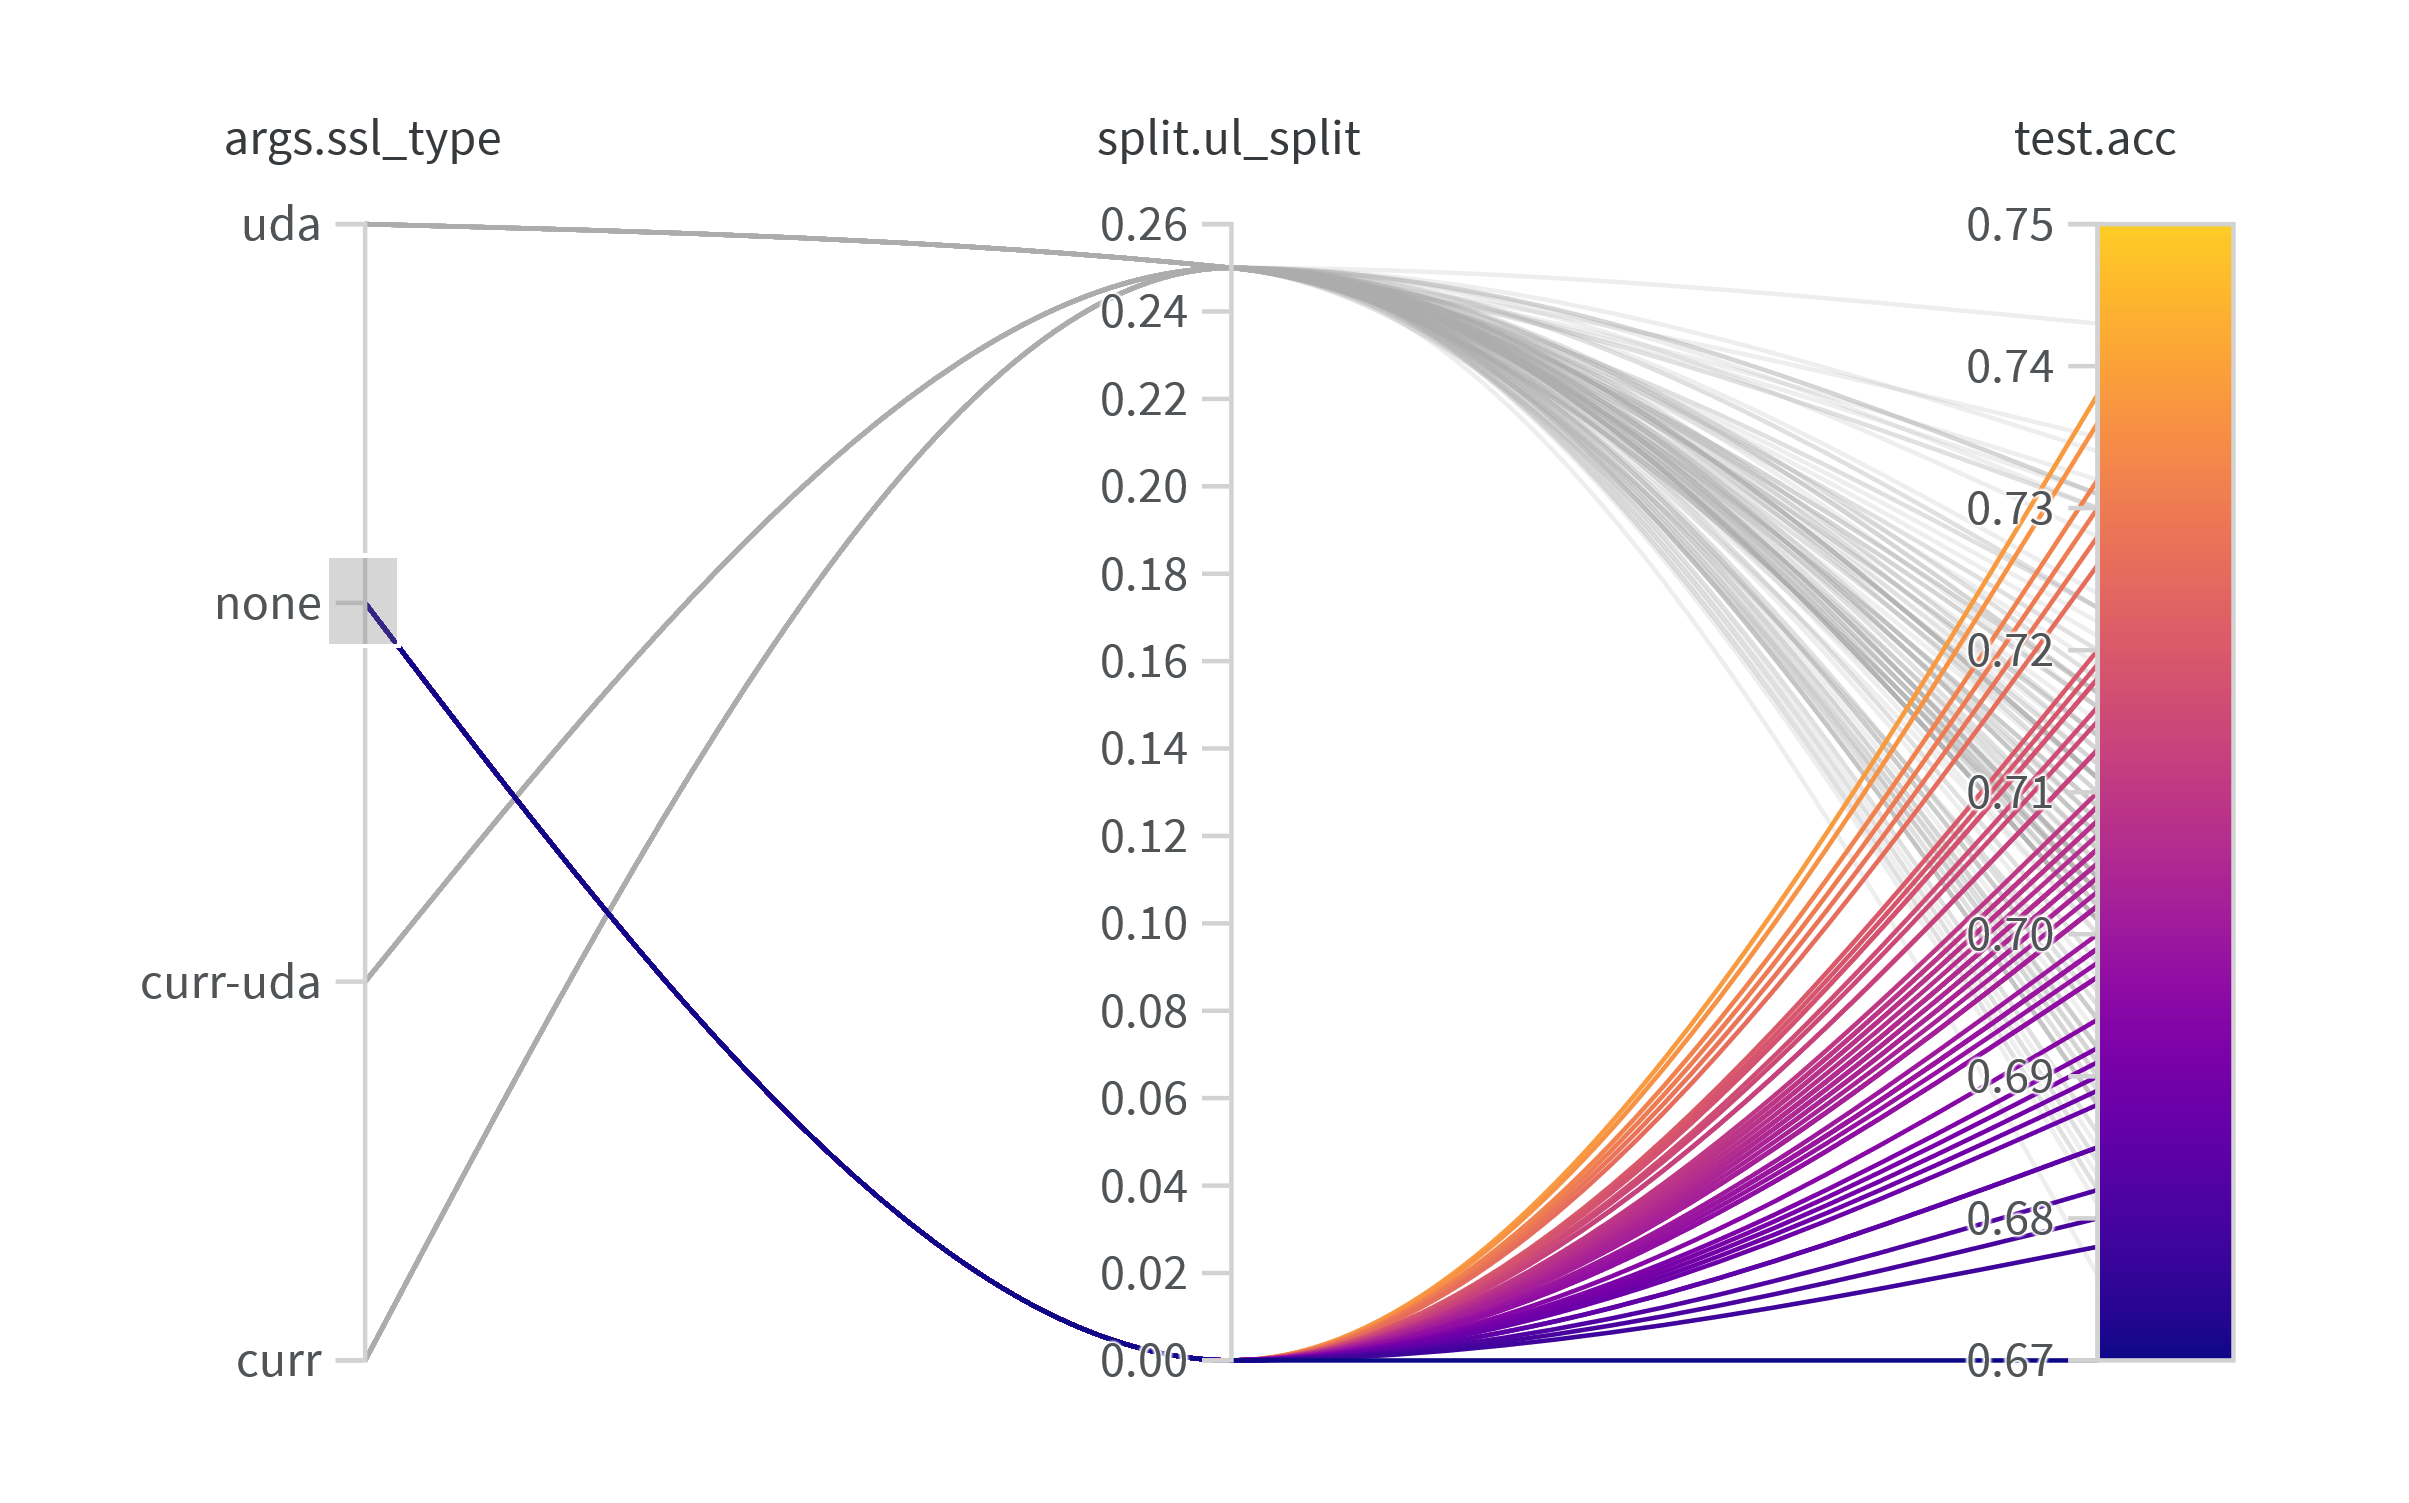
\includegraphics[width=0.48\columnwidth]{par_coords_jannis_mlp_icr_l_split_high_none.png}
  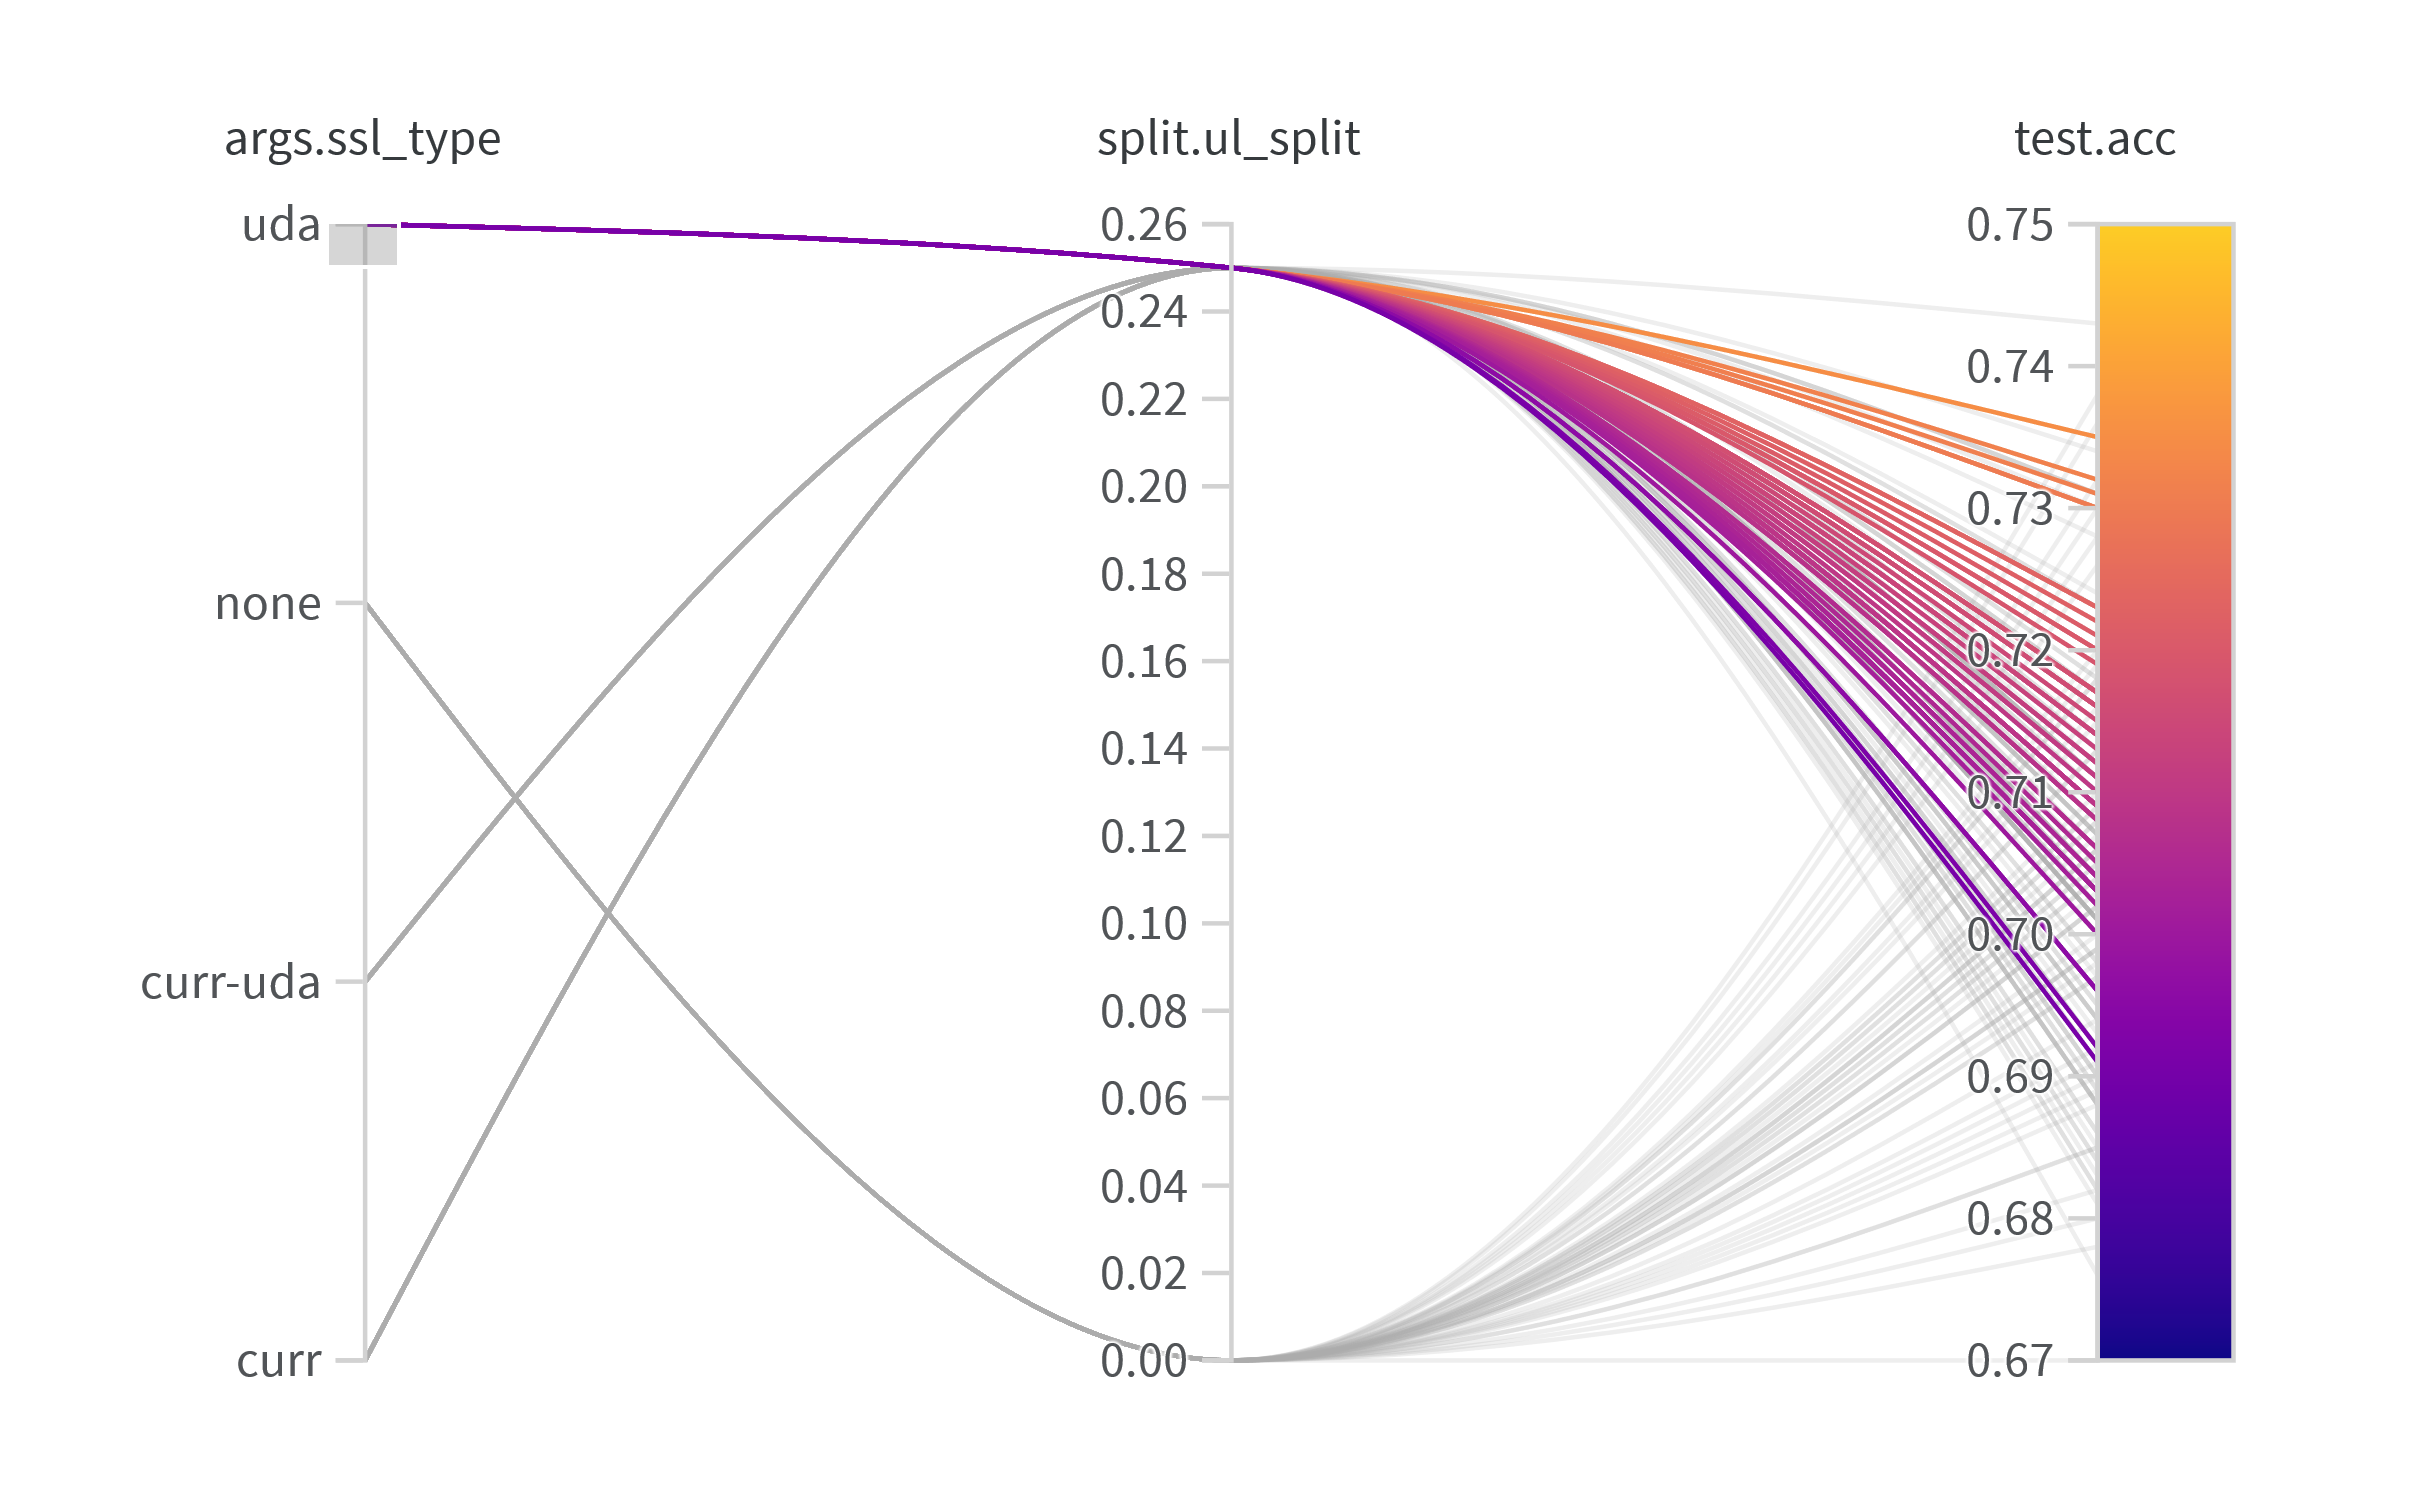
\includegraphics[width=0.48\columnwidth]{par_coords_jannis_mlp_icr_l_split_high_uda.png}
  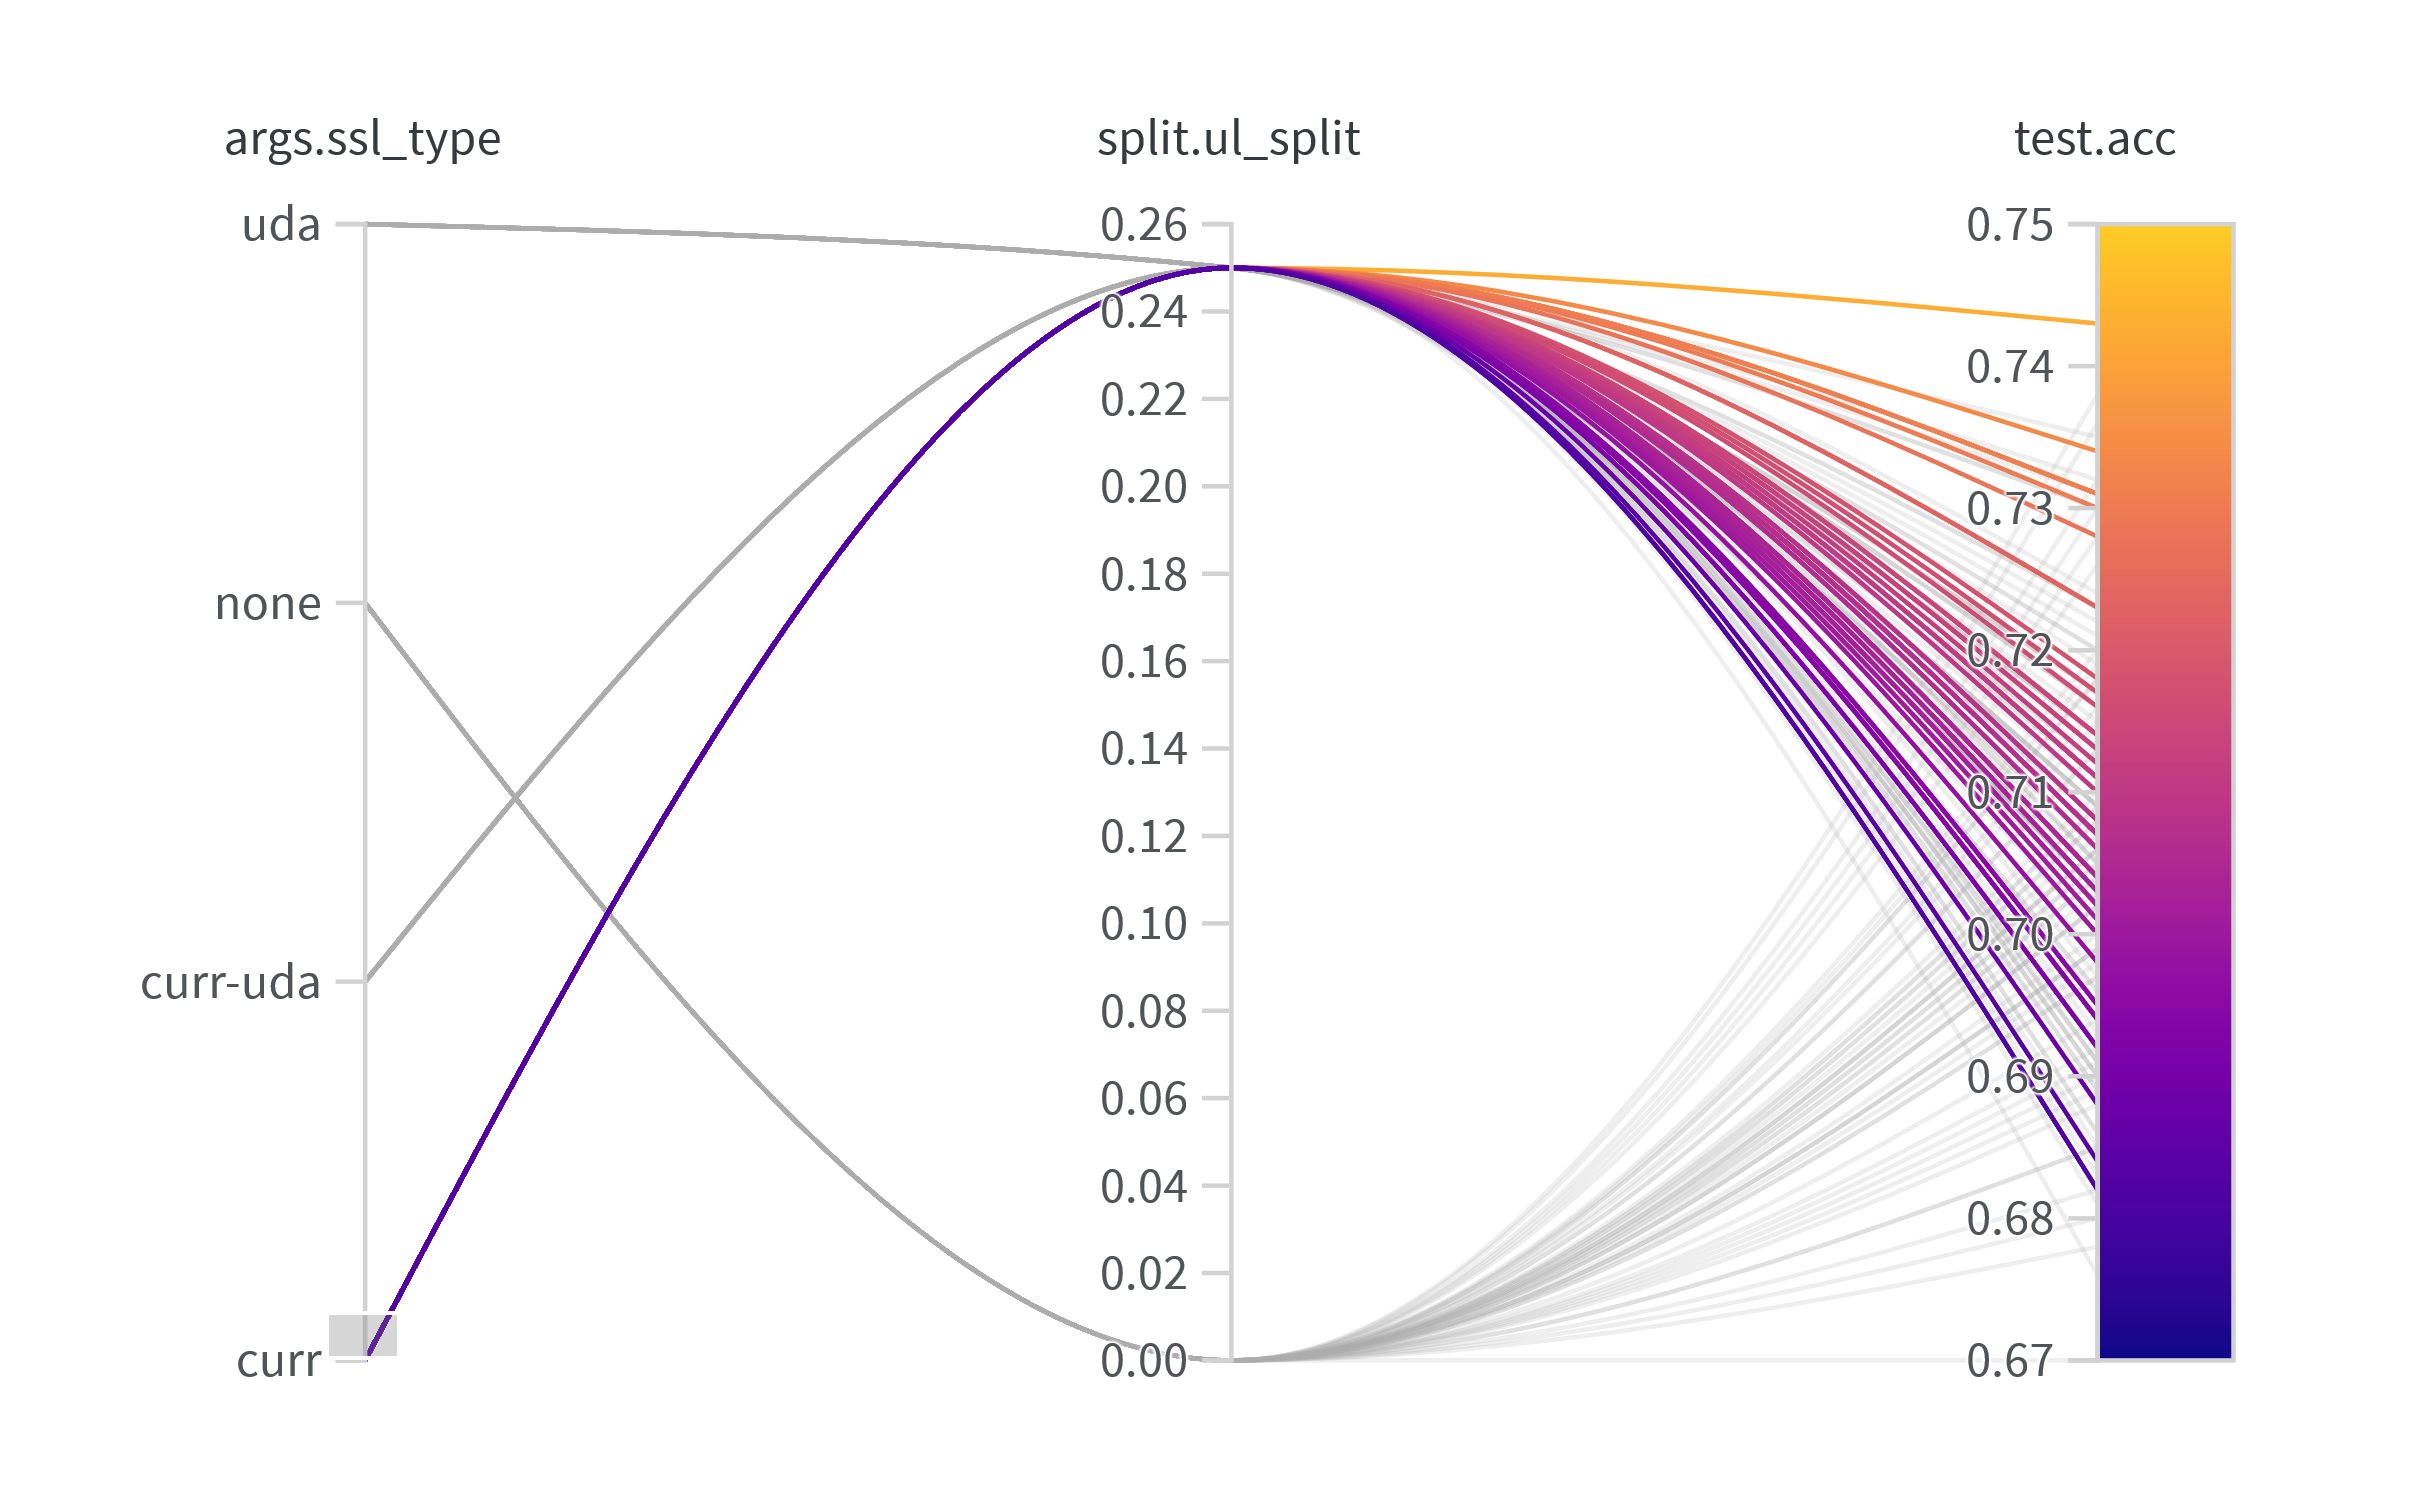
\includegraphics[width=0.48\columnwidth]{par_coords_jannis_mlp_icr_l_split_high_curr.png}
  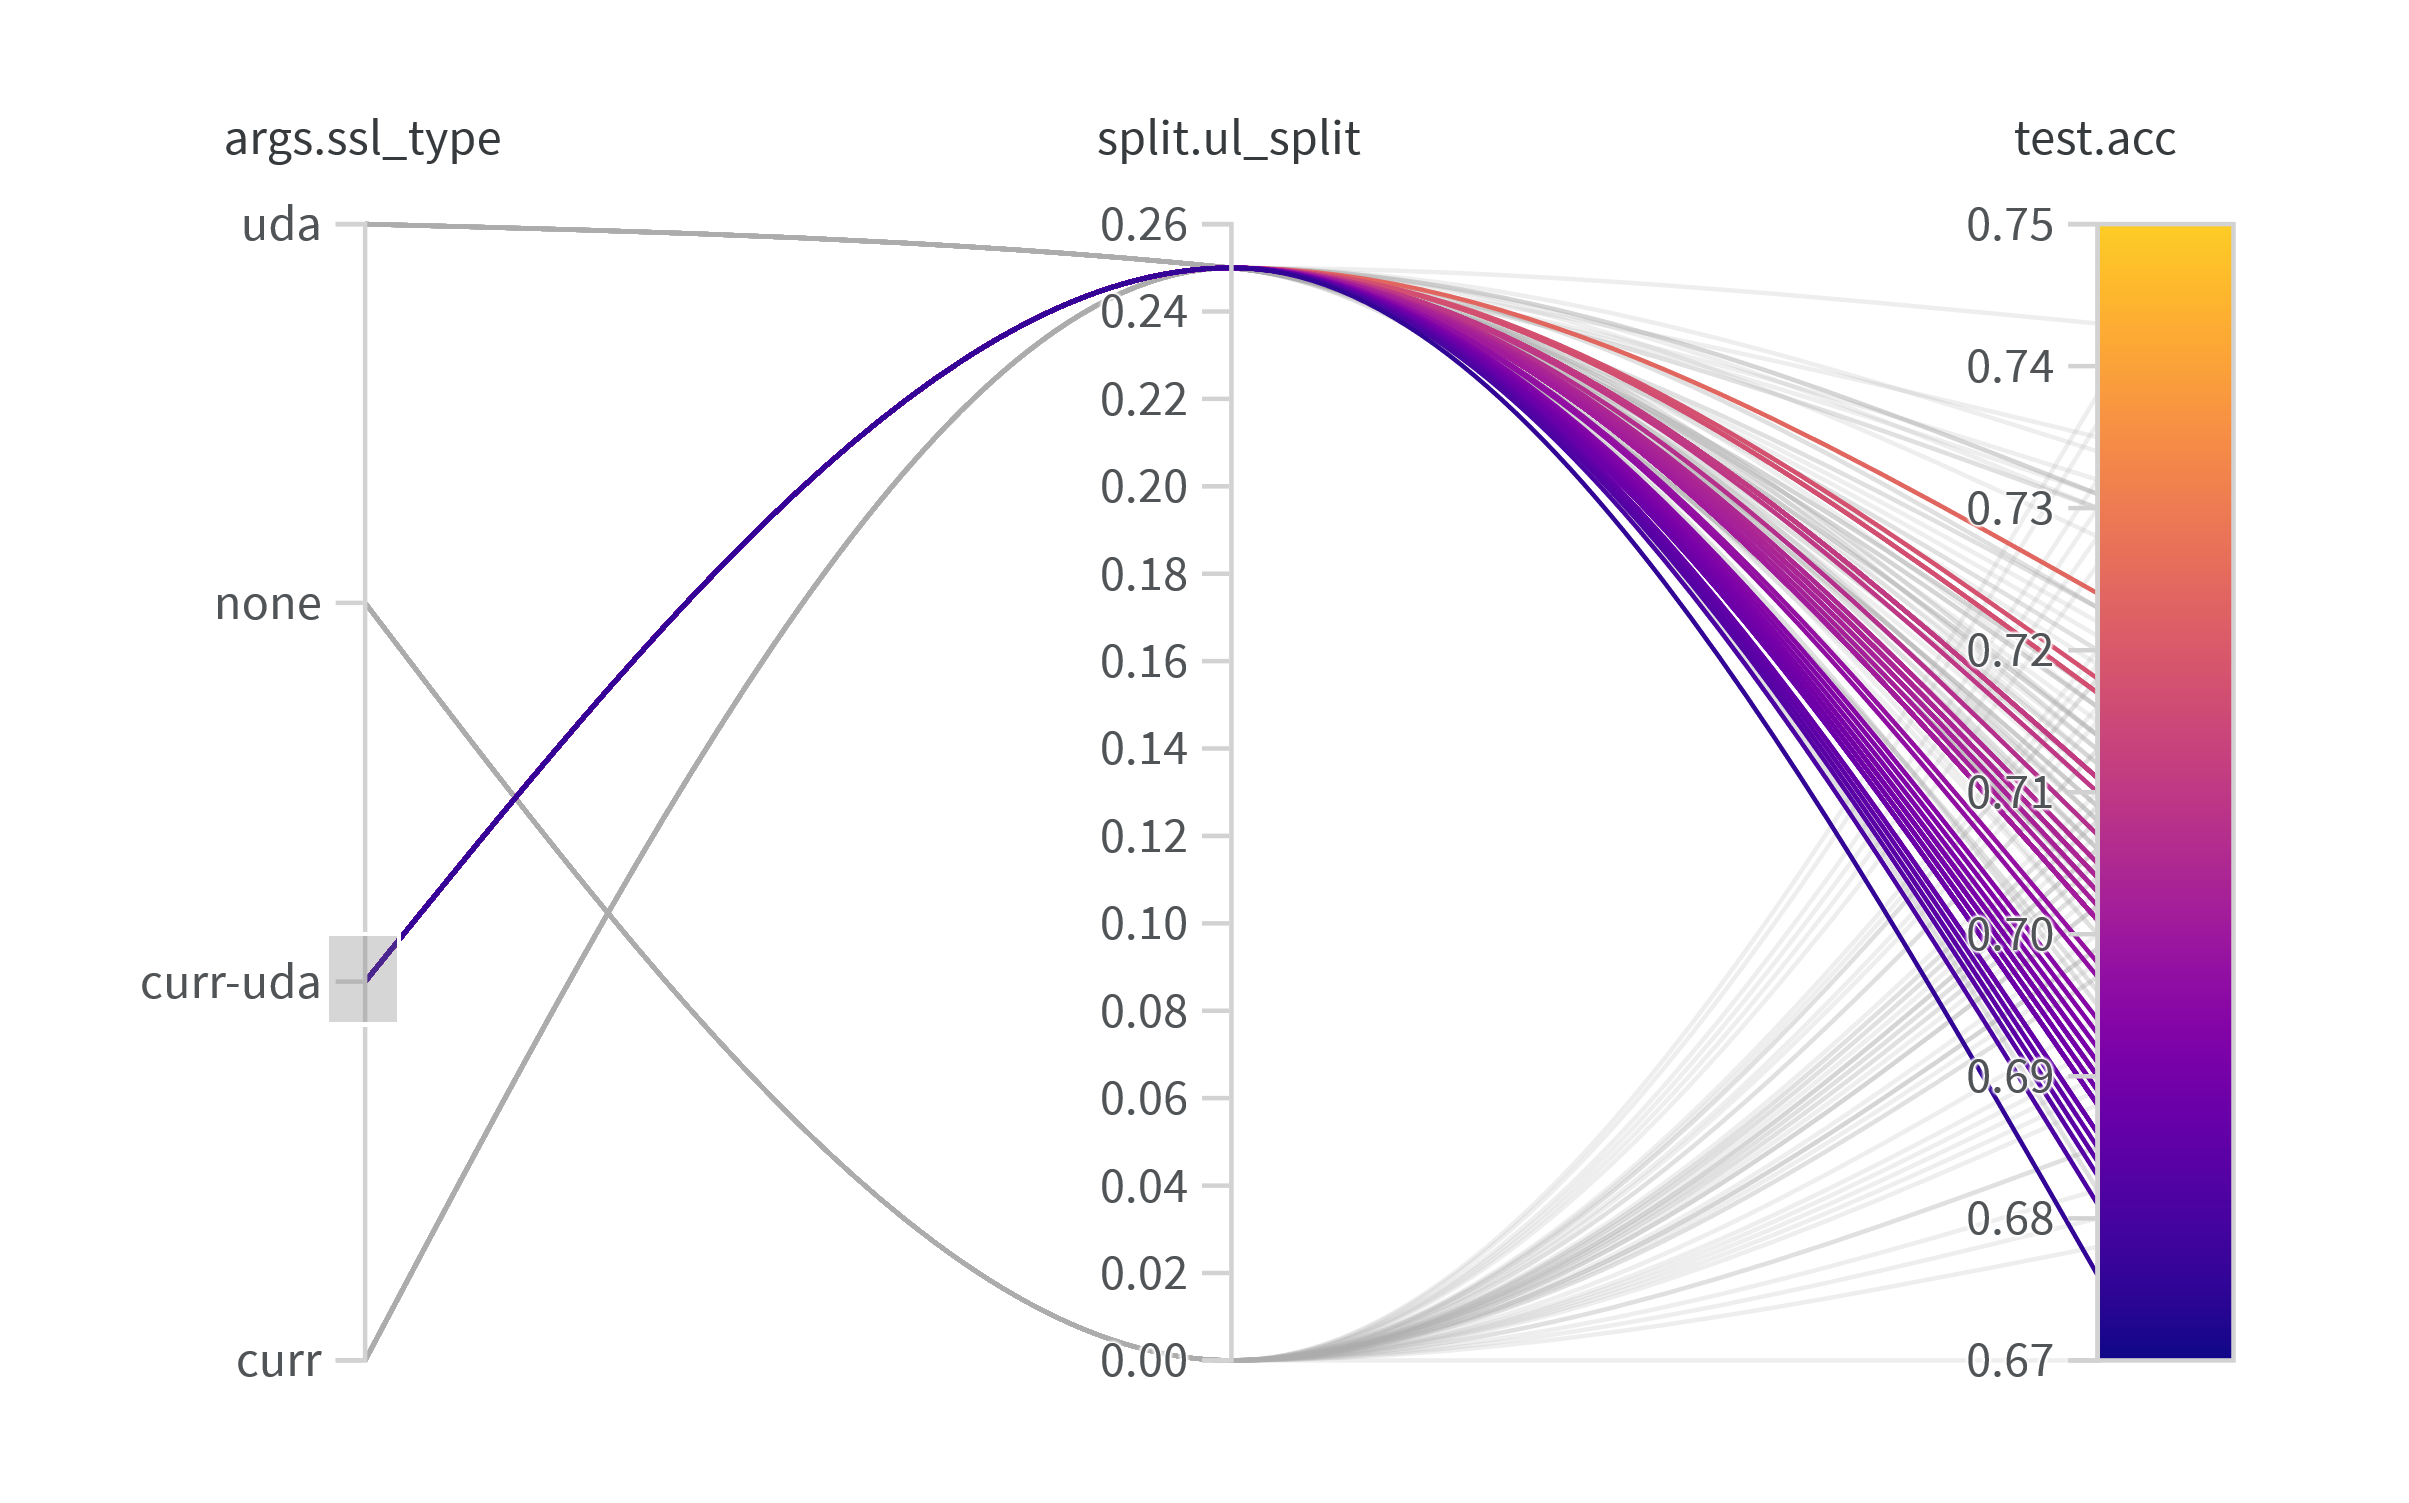
\includegraphics[width=0.48\columnwidth]{par_coords_jannis_mlp_icr_l_split_high_curr-uda.png}
  \caption{
    Parallel coordinate plots for \texttt{jannis}/\texttt{mlp} with
    \texttt{l\_split=0.25} (high-L).
    From top left to top right, \texttt{none} and \texttt{uda}; from bottom left to
    bottom right, \texttt{curr} and \texttt{curr-uda}.
    More interactive plots are available at
    {\small\url{https://api.wandb.ai/links/wei2912/3kho7181}}.
  }
  \label{fig:par_coords_jannis_mlp_icr_l_split_high}
\end{figure}

\clearpage
\paragraph{Stabilising effect of input consistency regularisation.}
Of the four methods tested, we observed that \texttt{uda} outperforms the other three
methods significantly, especially in the low-L regime (see Figure
\ref{fig:par_coords_jannis_mlp_icr_l_split_low}).
In fact, UDA had a stabilising effect on the test accuracy in both the low-L and high-L
regime, especially when applied to curriculum self-training in \texttt{curr-uda}.

\paragraph{Underperformance of curriculum self-training w/ UDA.}
Strangely, despite the stabilising effect of UDA and its strong performance against
the SL model, \texttt{curr-uda} underperforms compared to \texttt{uda}, with most
\texttt{uda} runs performing at least as well as \texttt{curr-uda} runs.
In the low-L regime, \texttt{uda} achieved test accuracies up to 72\%, while
the best performance of \texttt{curr-uda} is below 69\% (see Figure
\ref{fig:par_coords_jannis_mlp_icr_l_split_low}).

Speculatively, this might possibly be a consequence of the SCARF-style corruptions
discarding 60\% of features, which may lead to pseudolabels that encourage models to
rely on fewer features.
This makes the final model more robust to noise, but also restricts the best performance
attainable.
It remains to be seen if tuning the feature corruption rate of 60\% can lead to improved
performance.

\section{Conclusion}

\paragraph{Preliminary findings.}
The findings of the report can be summarised as follows: \begin{enumerate}
  \item Tree-based models continue to dominate across data regimes, although we find
  that MLPs may significantly under/overperform on different tabular datasets. (Section
  \ref{sec:overall-perf})
  \item Curriculum self-training without input consistency regularisation is prone to
  collapsing, with runs occasionally performing as well as random guessing. (Section
  \ref{sec:det_anal_jannis_mlp})
  \item Applying UDA with SCARF-style corruptions stabilises model performance, even
  outperforming SL models and reducing the frequency of collapse in curriculum
  self-training.
  However, curriculum self-training with UDA underperforms compared to UDA alone.
  (Section \ref{sec:icr_jannis_mlp})
\end{enumerate}

\paragraph{Limitations.}
Due to the complexity of dealing with tabular data and low-data settings, there are
several limitations in our experiments: \begin{enumerate}
  \item The high variability of tabular datasets demands more extensive benchmarking.
  \item Other hyperparameters might influence the collapsing phenomenon of curriculum
  self-training on MLPs, e.g. model depth or architecture.
  \item Curriculum self-training might not be the best option for low-L data regimes,
  and it is possible that carefully selected parameters for threshold self-training may
  yield better results.
  \item Other kinds of data augmentations besides SCARF-style corruptions may be more
  suitable for UDA on tabular data.
\end{enumerate}

\printbibliography

\appendix

\section{Hyperparameter Sweep Plots}
\label{sec:hyperparams_sweep_plots}

\begin{table}[htbp]
  \centering
  \caption{Hyperparameter search space for \texttt{hgbt}.}
  \label{tab:hyperparams_spaces_hgbt}
  \small
  \begin{tabular}{ccc}
    \toprule
    \texttt{lr} & \texttt{max\_depth} & \small\texttt{min\_samples\_leaf} \\
    \midrule
    0.05..0.5 (\texttt{step=0.05})
    & \texttt{None}, 2, 3, 4
    & 1..5 (\texttt{log=True}) \\
    \bottomrule
  \end{tabular}
\end{table}

\begin{table}[htbp]
  \centering
  \caption{Hyperparameter search space for \texttt{mlp}.}
  \label{tab:hyperparams_spaces_mlp}
  \small
  \begin{tabular}{ccccc}
    \toprule
    \texttt{batch\_size} & \texttt{layer\_size} & \texttt{lr} & \texttt{n\_block} & \texttt{n\_iter} \\
    \midrule
    128
    & 64..256 (\texttt{step=64})
    & 0.004..0.04 (\texttt{step=0.004})
    & 4
    & 1000 \\
    \bottomrule
  \end{tabular}
\end{table}

\begin{table}[htbp]
  \centering
  \caption{Hyperparameter search space for \texttt{random-forest}.}
  \label{tab:hyperparams_spaces_random_forest}
  \small
  \begin{tabular}{ccc}
    \toprule
    \texttt{max\_depth} & \small\texttt{min\_samples\_leaf} & \texttt{n\_estimators} \\
    \midrule
    \texttt{None}, 2, 3, 4 & 1..5 (\texttt{log=True}) & 100 \\
    \bottomrule
  \end{tabular}
\end{table}

\begin{figure}[htbp]
  \centering
  \includesvg[width=0.8\columnwidth]{sweep_pareto/jannis_hgbt.svg}
  \includesvg[width=0.8\columnwidth]{sweep_pareto/jannis_mlp.svg}
  \includesvg[width=0.8\columnwidth]{sweep_pareto/jannis_random-forest.svg}
  \caption{
    Harmonic mean of test accuracy (acc.) over five splits, across different
    hyperparameter sweeps on \texttt{jannis}.
  }
  \label{fig:sweep_pareto_jannis}
\end{figure}

\begin{figure}[htbp]
  \centering
  \includesvg[width=0.8\columnwidth]{sweep_pareto/gas-drift-different-concentrations_hgbt.svg}
  \includesvg[width=0.8\columnwidth]{sweep_pareto/gas-drift-different-concentrations_mlp.svg}
  \includesvg[width=0.8\columnwidth]{sweep_pareto/gas-drift-different-concentrations_random-forest.svg}
  \caption{
    Harmonic mean of test accuracy (acc.) over five splits, across different
    hyperparameter sweeps on \texttt{gas-drift}.
  }
  \label{fig:sweep_pareto_gas-drift-different-concentrations}
\end{figure}

\begin{figure}[htbp]
  \centering
  \includesvg[width=0.8\columnwidth]{sweep_pareto/higgs_hgbt.svg}
  \includesvg[width=0.8\columnwidth]{sweep_pareto/higgs_mlp.svg}
  \includesvg[width=0.8\columnwidth]{sweep_pareto/higgs_random-forest.svg}
  \caption{
    Harmonic mean of test accuracy (acc.) over five splits, across different
    hyperparameter sweeps on \texttt{higgs}.
  }
  \label{fig:sweep_pareto_higgs}
\end{figure}

\begin{figure}[htbp]
  \centering
  \includesvg[width=0.8\columnwidth]{sweep_pareto/covertype_hgbt.svg}
  \includesvg[width=0.8\columnwidth]{sweep_pareto/covertype_mlp.svg}
  \includesvg[width=0.8\columnwidth]{sweep_pareto/covertype_random-forest.svg}
  \caption{
    Harmonic mean of test accuracy (acc.) over five splits, across different
    hyperparameter sweeps on \texttt{covertype}.
  }
  \label{fig:sweep_pareto_covertype}
\end{figure}

\end{document}
